\section{Vectors}

\begin{ILOssec}
    \item \ILOe
\end{ILOssec}

\subsection{Introduction to vectors}
\label{sec:vectors_intro}

\begin{learningoutcomes}
\item Identify vector quantities and scalar quantities
\item Define a position vector and vectors between points
\item Calculate the magnitude of vectors and normalise them
\end{learningoutcomes}

Figure \ref{fig:electrolysis} shows an electrolysis experiment with several quantities in the chamber highlighted. Some of these are represented by a \textbf{single number}, such as water \textbf{temperature} and \textbf{density}, or the \textbf{concentration} of Sodium ions and Chloride ions. These are are called \textbf{scalar} quantities. 

The sodium ions experience a \textbf{force} to the right. The chloride ions experience a force to the left. These forces give rise to \textbf{acceleration}. These have both \textbf{magnitude} and \textbf{direction}, and are called \textbf{vectors}.

\begin{figure}[ht]
    \centering
    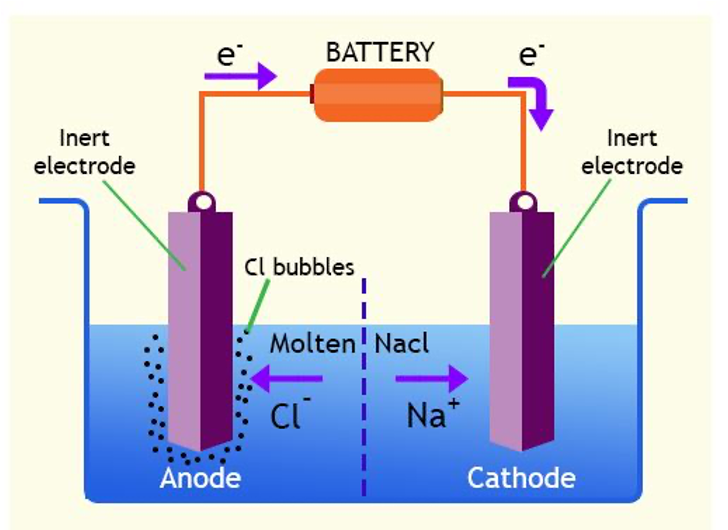
\includegraphics[width=0.5\linewidth]{Figures/Section4/41a_electrolysis.png}
    \caption{A sketch of an electrolysis chamber.}
    \label{fig:electrolysis}
\end{figure}

Some example scalar and vector quantities are given in \ref{tab:scalar_vector}.

\begin{table}[ht]
    \centering
    \begin{tabular}{c|c}
        Scalars & Vectors \\ \hline
        Mass & Force \\
        Volume & Acceleration \\
        Density & Momentum \\
        Energy & Concentration gradient \\
        Temperature & Temperature gradient \\
        \blankpar{Speed} & \blankpar{Velocity} \\
        \blankpar{Distance} & \blankpar{Displacement} \\
        \blankpar{Concentration} & \\
    \end{tabular}
    \caption{Some examples of scalars and vector quantities.}
    \label{tab:scalar_vector}
\end{table}

A vector is an entity giving the position of one point with respect to another. It is used to describe a physical quantity with a direction \emph{e.g.} 2 km north of here, 5 m s$^{-1}$ downwards. A vector has both \textbf{magnitude} and \textbf{direction}.

\textbf{Notation}.These notes will use bold and underlined letters (\emph{e.g.} $\myvec{a}$) for vectors. The vector from point $A$ to point $B$ is written as $\overrightarrow{AB}$. When handwritten, typically vectors are written as $\underline{a}$ or $\overrightarrow{a}$. When typed, often they are just written in bold e.g. $\myvec{a}$.

A vector is characterised by its magnitude (length) and direction, not by the position of the head and tail. In figure \ref{fig:vec_sketch}(a) vectors $\myvec{a}$ are all the same vector but $\myvec{b}$ is a different vector.

Two vectors are said to be \textbf{parallel} if they point in the same direction, even if the magnitudes (lengths) are different. The three vectors shown in \ref{fig:vec_sketch}(b) are parallel.
\begin{figure}[ht]
    \centering
    \subfig{0.4}{Figures/Section4/41b_vectors.png}{$\myvec{a}$ are all the same vector.}
    \subfig{0.4}{Figures/Section4/41c_parallel.png}{These vectors are parallel.}
    \caption{}
    \label{fig:vec_sketch}
\end{figure}

The vectors $\myvec{i}$, $\myvec{j}$, and $\myvec{k}$ are vectors of length 1 (\emph{i.e.}\textbf{unit vectors}) that point in the positive $x$, $y$, and $z$ directions (figure \ref{fig:ijk}(a)). A vector can be expressed in terms of $\myvec{i}$, $\myvec{j}$, and $\myvec{k}$. Note, sometimes, unit vectors are written with a ``hat'' e.g. $\hat{\myvec{k}}$.

A vector representing a displacement of
\begin{itemize}
\item $a$ units in the $x$-direction
\item $b$ units in the $y$-direction
\item $c$ units in the $z$-direction
\end{itemize}
can be represented as $a\myvec{i}+b\myvec{j}+c\myvec{k}$. For example, the vector $\myvec{v}=2\myvec{i}+\myvec{j}+4\myvec{k}$ (shown in figure \ref{fig:ijk}(b)) goes
\begin{itemize}
\item 2 units to the right,
\item 1 unit back (into the page),
\item 4 units up.
\end{itemize}
\begin{figure}[ht]
    \centering
    \subfig{0.4}{Figures/Section4/41d_ijk.png}{Sketch of the $\myvec{i}$, $\myvec{j}$, $\myvec{k}$ vectors.}
    \subfig{0.35}{Figures/Section4/41e_ijk_example.png}{The vector $\myvec{v}=2\myvec{i}+\myvec{j}+4\myvec{k}$}
    \caption{}
    \label{fig:ijk}
\end{figure}


Alternatively, we can denote this as
\[
\myvec{v}=\begin{pmatrix}2\\1\\4\end{pmatrix}.
\]

\textbf{Position Vector.} The vector from the origin to a point is referred to as the \textbf{position vector} of that point. For example, the point $P=(4,3)$ has position vector $\myvec{p}=4\myvec{i}+3\myvec{j}$ (figure \ref{fig:vec_types}(a)).

\textbf{Vector from point to point.} The vector from the point $A$ with coordinates $(a_x,a_y,a_z)$ to a point $B$ with coordinates $(b_x,b_y,b_z)$ is given by
\begin{equation}
\overrightarrow{AB}=(b_x-a_x)\myvec{i}+(b_y-a_y)\myvec{j}+(b_z-a_z)\myvec{k}
=\myvec{b}-\myvec{a}.
\end{equation}
\emph{E.g.} the vector from $(2,6,-1)$ to $(3,4,8)$ is
\[
(3-2)\myvec{i}+(4-6)\myvec{j}+(8+1)\myvec{k}
=\myvec{i}-2\myvec{j}+9\myvec{k}.
\]

This is the same in two dimensions. E.g. vector from $A=(2,6)$ to $B=(3,4)$ is $\overrightarrow{AB}=\myvec{i}-2\myvec{j}$ ((figure \ref{fig:vec_types}(b))).

\textbf{Magnitude of a Vector.} The magnitude, or length, of a vector, such as $\myvec{a}=a_x\myvec{i}+a_y\myvec{j}+a_z\myvec{k}$ is given by
\begin{equation}
\lvert\myvec{a}\rvert=\sqrt{a_x^2+a_y^2+a_z^2}.    
\end{equation}
\textit{E.g.} the magnitude of $\myvec{b}=4\myvec{i}+\myvec{j}-8\myvec{k}$ is
\[
\lvert\myvec{b}\rvert=\sqrt{4^2+1^2+(-8)^2}=\sqrt{16+1+64}=\sqrt{81}=9.
\]
In two dimensions, the formula is the same (with $a_z=0$). For example, the vector from $A=(2,9)$ to $B=(14,4)$ is given by $\myvec{p}=12\myvec{i}-5\myvec{j}$ ((figure \ref{fig:vec_types}(c))). The magnitude of $\myvec{p}$ is
\[
\lvert\myvec{p}\rvert=\sqrt{12^2+5^2}=\sqrt{169}=13.
\]
\begin{figure}[ht]
    \centering
    \subfig{0.34}{Figures/Section4/41f_2d_vector.png}{Position vector}
    \hfill
    \subfig{0.28}{Figures/Section4/41g_p2p_vector.png}{Point-to-point vector}
    \hfill
    \subfig{0.34}{Figures/Section4/41h_mag_vector.png}{Magnitude of a vector}
    \caption{Examples of various vector definitions}
    \label{fig:vec_types}
\end{figure}


\textbf{Vector scaling and normalisation.} Suppose we have a vector $\myvec{a}$ and we want to find a vector $\myvec{b}$ with the same direction as $\myvec{a}$ but with a given magnitude $m$. Then
\begin{align}
    \myvec{b}=m\frac{\myvec{a}}{\lvert\myvec{a}\rvert}.
\end{align}
A special case is ``normalisation'' of $\myvec{a}$, where we find the ``unit vector'' parallel to $\myvec{a}$, given by
\begin{equation}
  \hat{\myvec{a}}=\frac{1}{\lvert\myvec{a}\rvert}\myvec{a}.  
\end{equation}
The vector $\hat{\myvec{a}}$ has the same direction as $\myvec{a}$, but with magnitude 1.

\begin{example}[Lecture]
Given the points $A=(4,2,11)$ and $B=(6,5,5)$ find
\begin{itemize}
\item The position vector $\myvec{a}$ of the point $A$
\item The vector $\overrightarrow{AB}$
\item The magnitude of vector $\overrightarrow{AB}$
\item The vector $\myvec{v}$ parallel to $\overrightarrow{AB}$ with magnitude 2
\end{itemize}
\end{example}
\begin{solution}
\begin{itemize}
    \item $\myvec{a}=\blank{4\myvec{i}+2\myvec{j}+11\myvec{k}}$.
    \item $\overrightarrow{AB} = \blank{\myvec{b}-\myvec{a}}
        = \blank{(6-4)\myvec{i}+(5-2)\myvec{j}+(5-11)\myvec{k}
        =2\myvec{i}+3\myvec{j}-6\myvec{k}.}$
    \item $\lvert\overrightarrow{AB}\rvert =\blank{\sqrt{2^2+3^2+(-6)^2} =\sqrt{4+9+36}=7}$.
    \item $\myvec{v}= \blank{2\frac{\overrightarrow{AB}}{\lvert\overrightarrow{AB}\rvert}}
    = \blank{\frac{2}{7}\left(2\myvec{i}+3\myvec{j}-6\myvec{k}\right)
    = \frac{4}{7}\myvec{i}+\frac{6}{7}\myvec{j}-\frac{12}{7}\myvec{k}}$.
\end{itemize}

\end{solution}

\begin{recap}{\ref{sec:vectors_intro}}
\item \textbf{Vectors}, unlike scalars, have a \textbf{direction} as well as a magnitude.
\item Vectors can be written in the form
\[
a\myvec{i}+b\myvec{j}+c\myvec{k}
\qquad\text{or}\qquad
\begin{pmatrix}a\\b\\c\end{pmatrix}.
\]
\item The position vector of a point $P=(x,y,z)$ is
\[
\myvec{p}=x\myvec{i}+y\myvec{j}+z\myvec{k}.
\]
\item To calculate the vector from $A$ to $B$, subtract the coordinates of $A$ from those of $B$.
\end{recap}

\subsection{Additive operations on vectors}
\label{sec:vector_add}

\begin{learningoutcomes}
\item Perform addition and subtraction of vector quantities
\item Multiply vectors by scalar quantities
\end{learningoutcomes}
%Continue here
\textbf{Addition of Vectors.} The sum of two vectors is another vector. To find $\myvec{a}+\myvec{b}$, put the `tail' of $\myvec{b}$ next to the head of $\myvec{a}$. Then $\myvec{a}+\myvec{b}$ joins the `tail' of $\myvec{a}$ to the head of $\myvec{b}$ (figure \ref{fig:vec_add}(a)). 

Note that $\myvec{a}+\myvec{b}$ and $\myvec{b}+\myvec{a}$ are equal: \emph{i.e.} addition of vectors is \textbf{commutative} (figure \ref{fig:vec_add}(b)). Furthermore, $(\myvec{a}+\myvec{b})+\myvec{c}$ and $\myvec{a}+(\myvec{b}+\myvec{c})$ are equal: \emph{i.e.} addition of vectors is \textbf{associative}  (figure \ref{fig:vec_add}(c)).

\begin{figure}
    \centering
    \subfig{0.3}{Figures/Section4/42a_vector_add.png}{Vector addition.}
    \subfig{0.3}{Figures/Section4/42b_vector_add2.png}{Commutative property.}
    \subfig{0.38}{Figures/Section4/42c_vector_add3.png}{Associative property.}
    \caption{Geometric representations of vector addition.}
    \label{fig:vec_add}
\end{figure}

To add two vectors, simply add the components. Take $\myvec{a}=2\myvec{i}-\myvec{j}+3\myvec{k}$ and $\myvec{b}=3\myvec{i}+2\myvec{j}-4\myvec{k}$. Then,
\begin{align*}
\myvec{a}+\myvec{b} &=(2+3)\myvec{i}+((-1)+2)\myvec{j}+(3+(-4))\myvec{k} \\
&=5\myvec{i}+\myvec{j}-\myvec{k}.
\end{align*}

\textbf{Subtraction of Vectors.} The difference between vectors $\myvec{a}-\myvec{b}$, is also a vector. To find $\myvec{a}-\myvec{b}$, put the `tails' next to each other and join the head of $\myvec{b}$ to the head of $\myvec{a}$ (figure \ref{fig:vec_sub}).
\begin{figure}[ht]
    \centering
    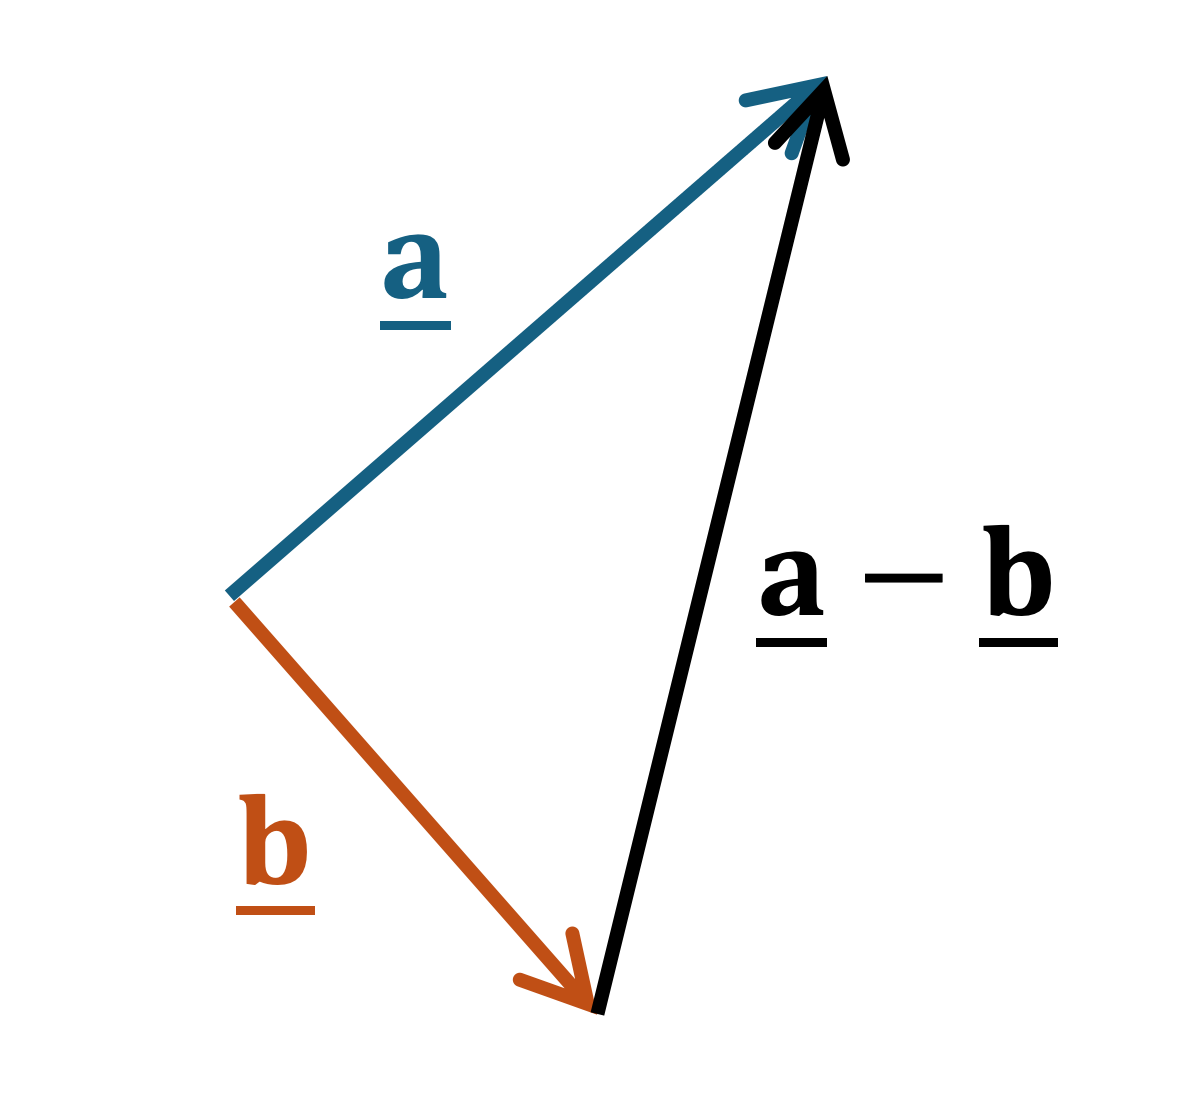
\includegraphics[width=0.2\linewidth]{Figures/Section4/42d_vector_subtract.png}
    \caption{Geometric representation of vector subtraction}
    \label{fig:vec_sub}
\end{figure}


To subtract the vectors, simply subtract the components. Take $\myvec{a}=2\myvec{i}-\myvec{j}+3\myvec{k}$ and $\myvec{b}=3\myvec{i}+2\myvec{j}-4\myvec{k}$. Then,
\begin{align*}
\myvec{a}-\myvec{b} &=(2-3)\myvec{i}+((-1)-2)\myvec{j}+(3-(-4))\myvec{k} \\
&=-\myvec{i}-3\myvec{j}+7\myvec{k}.
\end{align*}

\textbf{Multiplication of Vectors by Scalars.} A vector $\myvec{a}$ can be multiplied by a scalar $\lambda$ (a number). The result is a vector, \emph{e.g.} $\myvec{b}=\lambda\myvec{a}$.
\begin{itemize}
\item For positive $\lambda$ the result has the same direction as the original and the magnitude changes.
\item For negative $\lambda$, the result points in the opposite direction (figure \ref{fig:scalar_mult}).
\end{itemize}
The resulting vector has all of its components multiplied by $\lambda$. So, if $\myvec{a}=a_x\myvec{i}+a_y\myvec{j}+a_z\myvec{k}$ then
\begin{equation}
\lambda\myvec{a}=\lambda a_x\myvec{i}+\lambda a_y\myvec{j}+\lambda a_z\myvec{k} \,.    
\end{equation}

\begin{figure}[ht]
    \centering
    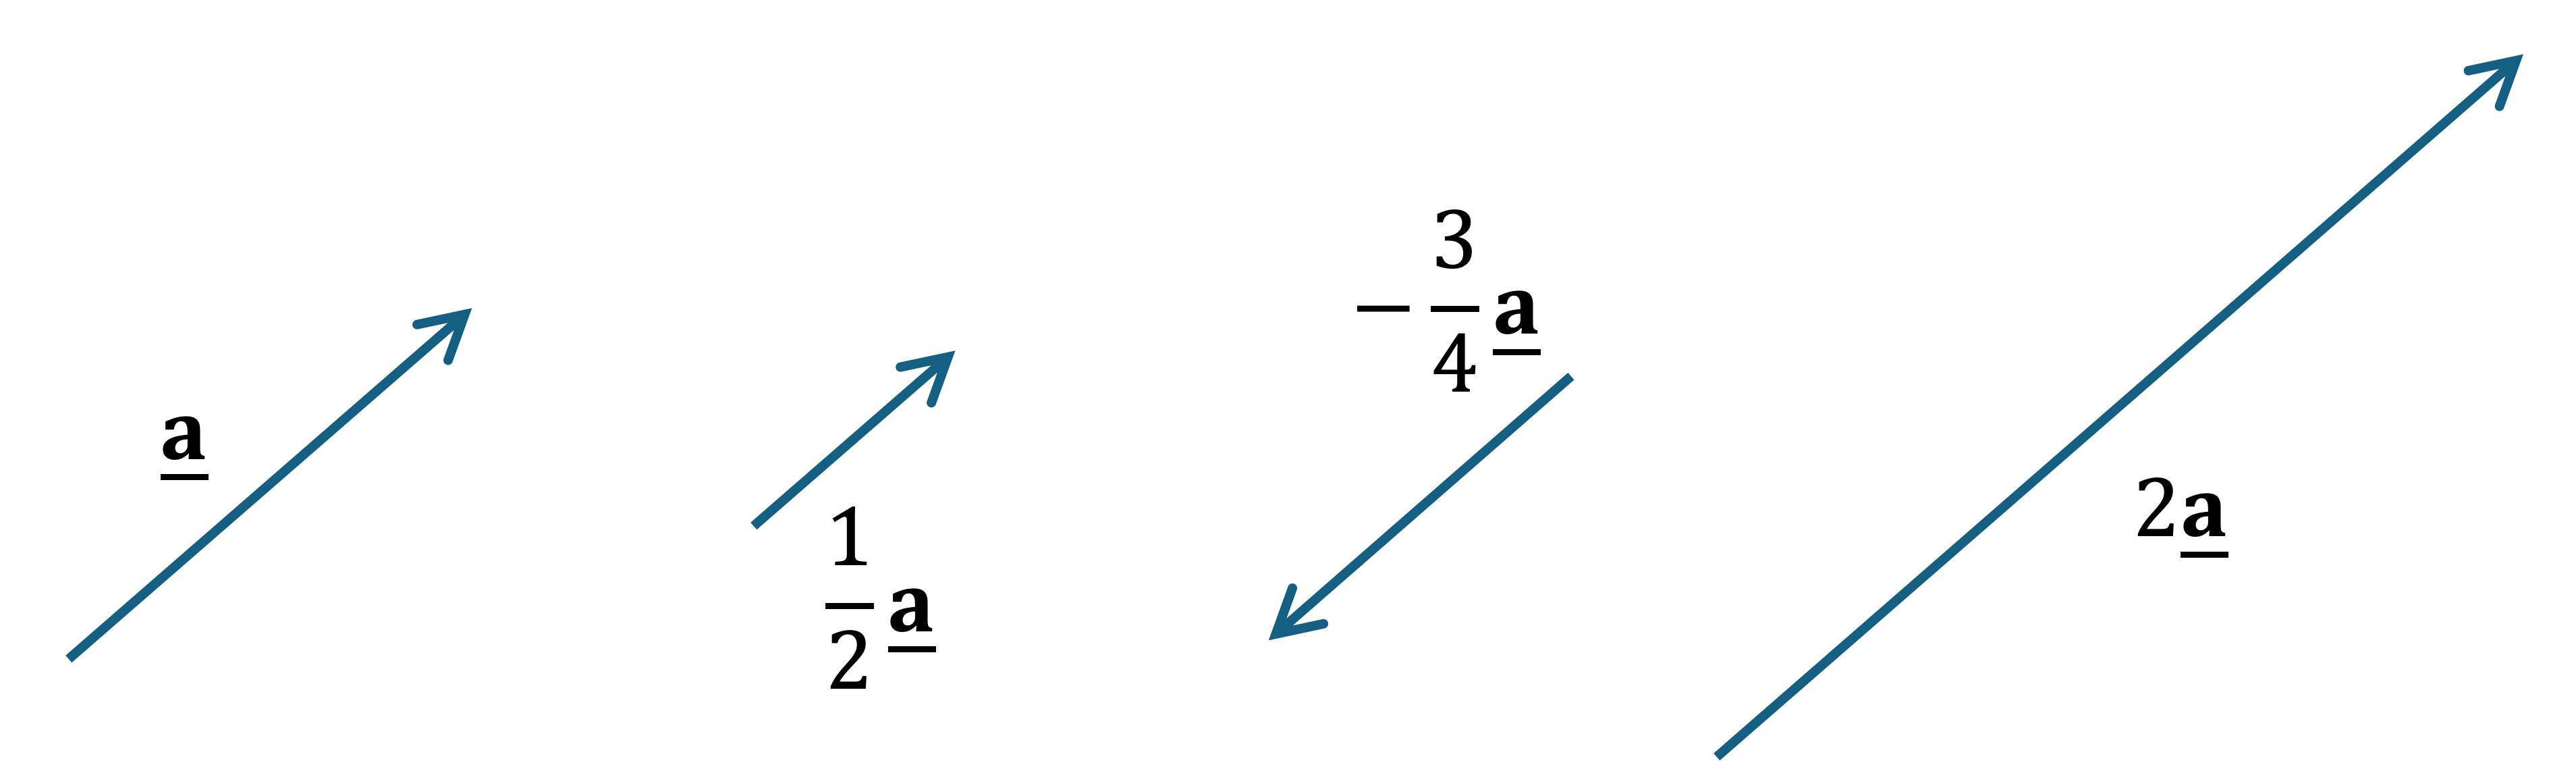
\includegraphics[width=0.8\linewidth]{Figures/Section4/42e_scalar_mult.png}
    \caption{Different scalar multiples of the vector $\myvec{a}$.}
    \label{fig:scalar_mult}
\end{figure}

\emph{E.g.} Take $\myvec{a}=2\myvec{i}-\myvec{j}+3\myvec{k}$ and $\lambda=5$, then
\begin{align*}
\myvec{b} = \lambda\myvec{a} &=5(2\myvec{i}-\myvec{j}+3\myvec{k})\\
&=10\myvec{i}-5\myvec{j}+15\myvec{k}.
\end{align*}

\textbf{Distributive Laws.} Note the distributive properties of multiplication by a scalar.
\begin{align}
    \lambda\myvec{a}+\lambda\myvec{b}&=\lambda(\myvec{a}+\myvec{b}),\\
    \lambda\myvec{a}+\mu\myvec{a}&=(\lambda+\mu)\myvec{a}.
\end{align}

\begin{example}[Lecture]
Calculate the vectors
\[
\myvec{u}=3\myvec{a}+5\myvec{a}
\]
and
\[
\myvec{v}=\frac{1}{4}\myvec{u}+2\myvec{b},
\]
where
\[
\myvec{a}=\myvec{i}-2\myvec{k}
\qquad\text{and}\qquad
\myvec{b}=\frac{1}{2}\myvec{j}+3\myvec{k}.
\]
\end{example}

\begin{solution}
\[
\myvec{u}=3\myvec{a}+5\myvec{a}=\blank{8\myvec{a}
=8\myvec{i}-16\myvec{k}}.
\]
\begin{align*}
\myvec{v}=\frac{1}{4}\myvec{u}+2\myvec{b}
&=\blank{\frac{1}{4}(8\myvec{i}-16\myvec{k})
+2\left(\frac{1}{2}\myvec{j}+3\myvec{k}\right)}
&=2\myvec{i}+\myvec{j}+2\myvec{k}.
\end{align*}
\end{solution}

\begin{example}[Video]
A ``Janus particle'' converts chemical energy into motion to ``swim'' on a surface. In an experiment the $(x,y)$ position is measured every 10 seconds. One particle starts at $A=(2,3)$ [$\mu$m], at the next measurement it is at $B=(5,2)$ [$\mu$m].
\begin{enumerate}[label=(\alph*)]
    \item Assuming it travels in a straight line, what is its velocity the first 10s of the experiment?
    \item  The particle changes direction, travelling for the next 10s with average velocity
    \[
        \myvec{v}=-0.1\myvec{i}+0.4\myvec{j}\;\mu\mathrm{m/s}.
    \]
    What is its position at the next measurement?
    \item It continues to travel at the same velocity for the next 20s, how far is it from its starting point (40s into the experiment)?
\end{enumerate}
\begin{center}
    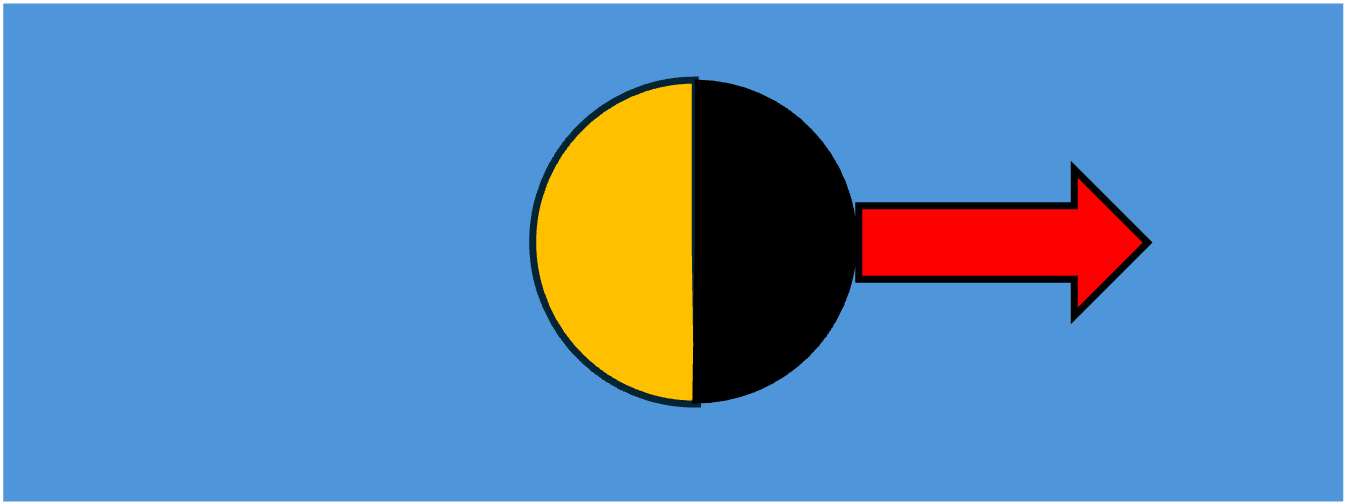
\includegraphics[width=0.4\textwidth,alt={Sketch of a janus particle.}]{Figures/Section4/Ex422.png}
\end{center}
\end{example}

\begin{solution}
\begin{enumerate}[label=(\alph*)]
\item Define position vectors $\myvec{a}=2\myvec{i}+3\myvec{j}$ and $\myvec{b}=5\myvec{i}+2\myvec{j}$. \par
Velocity = displacement/time. The displacement is
\[
\overrightarrow{AB}=\blank{(5-2)\myvec{i}+(2-3)\myvec{j}=3\myvec{i}-\myvec{j}}\quad[\mu\mathrm{m}]
\]
so velocity is $\myvec{u}=\blank{0.3\myvec{i}-0.1\myvec{j}}$ $[\mu\mathrm{m/s}]$
\item $\myvec{v}=-0.1\myvec{i}+0.4\myvec{j}$ mm/s so after 10s its position will be
\[
\myvec{c}=\myvec{b}+10\myvec{v}
=\blank{(5-1)\myvec{i}+(2+4)\myvec{j}=4\myvec{i}+6\myvec{j}}\quad[\mu\mathrm{m}]
\]
\item After 20s more its position is
\[
\myvec{d}=\myvec{c}+20\myvec{v}
=\blank{(4-3)\myvec{i}+(6+12)\myvec{j}=\myvec{i}+18\myvec{j}}\quad[\mu\mathrm{m}]
\]
The distance from the starting point is
\[
|\overrightarrow{AD}|=|\myvec{d}-\myvec{a}|
=\blank{|-\myvec{i}+15\myvec{j}|=\sqrt{1+15^2}=\sqrt{226}\approx15.03}\quad[\mathrm{mm}]
\]
\end{enumerate}
\end{solution}

\textbf{Additive properties of vectors vs. scalars.} Therefore, additive operations on vectors share all the same properties as additive operations on scalars, they are
\begin{itemize}
\item Commutative
\item Associative
\item Distributive
\end{itemize}

However, a \textbf{scalar and vector cannot be added together} directly, as they are fundamentally different objects.

\begin{recap}{\ref{sec:vector_add}}
\item Vectors can be added / subtracted by \textbf{adding / subtracting their components}. The result is a vector.
\item To multiply a vector by a scalar, \textbf{multiply each component} of the vector by the scalar. The result is a vector that is \textbf{(anti-)parallel to the original}.
\item \textbf{Scalars cannot be added to vectors} directly, as they are fundamentally different objects.
\end{recap}

\subsection{The scalar product}
\label{sec:scalar_prod}

\begin{learningoutcomes}
\item Define the scalar product of two vectors in terms of their magnitude and angle
\item Calculate the scalar product of two vectors
\end{learningoutcomes}

\textbf{The Scalar Product.} Two vectors may be multiplied to give a scalar. The symbol $\boldsymbol{\cdot}$ is used to denote this kind of multiplication. The scalar product of vectors $\myvec{a}$ and $\myvec{b}$ is written as
\[
\myvec{a}\boldsymbol{\cdot}\myvec{b}.
\]
It is often pronounced as $\myvec{a}$ `dot' $\myvec{b}$ and is sometimes also referred to as the ``dot product''.

As the name suggests, the result of the scalar product is a \textbf{scalar}. Given two vectors, $\myvec{a}$ and $\myvec{b}$, the scalar product $\myvec{a}\boldsymbol{\cdot}\myvec{b}$ is defined as
\begin{equation}
    \myvec{a}\boldsymbol{\cdot}\myvec{b}
=\lvert\myvec{a}\rvert\lvert\myvec{b}\rvert\cos\theta,
\end{equation}
where $\theta$ is the angle between the vectors. It follows from the sign of $\cos\theta$ that if
\begin{itemize}
    \item $\myvec{a}$ and $\myvec{b}$ are separated by an \textbf{acute} angle $(-\pi/2<\theta<\pi/2)$, then $\myvec{a}\boldsymbol{\cdot}\myvec{b} > 0$;
    \item $\myvec{a}$ and $\myvec{b}$ are separated by an \textbf{obtuse} angle $(\pi/2 < |\theta| \leq \pi)$, then $\myvec{a}\boldsymbol{\cdot}\myvec{b} < 0$;
    \item $\myvec{a}$ and $\myvec{b}$ are separated by a \textbf{right} angle $(-\pi/2<\theta<\pi/2)$, then $\myvec{a}\boldsymbol{\cdot}\myvec{b} = 0$.
\end{itemize}
Two vectors at right angles are said to be \textbf{orthogonal} or \textbf{perpendicular}. The fact that the scalar product is zero is often used as a test of whether two vectors are perpendicular. 

Conversely, if two vectors are parallel, then $\cos\theta=1$ and so the scalar product is equal to the product of their magnitudes. A special case of this is the scalar product of a vector with itself
\[
\myvec{a}\boldsymbol{\cdot}\myvec{a}=\lvert\myvec{a}\rvert^2.
\]

\begin{example}[Lecture]
Given the vectors
\[
\myvec{a}=\myvec{i}+\myvec{j}
\qquad\text{and}\qquad
\myvec{b}=5\myvec{i},
\]
find the scalar product
\[
\myvec{a}\boldsymbol{\cdot}\myvec{b}.
\]
\end{example}

\begin{solution}
Calculate the scalar product using
\[
\myvec{a}\boldsymbol{\cdot}\myvec{b}
=\lvert\myvec{a}\rvert\lvert\myvec{b}\rvert\cos\theta.
\]

\[
\lvert\myvec{a}\rvert=\blank{\sqrt{1^2+1^2}=\sqrt{2},}
\qquad
\lvert\myvec{b}\rvert=\blank{\sqrt{5^2}=5.}
\]

By trig, the angle is given by
\[
\theta=\blank{\arctan\left(\frac{1}{1}\right)=\frac{\pi}{4}.}
\]
And so
\[
\cos\theta=\blank{\cos\left(\frac{\pi}{4}\right)=\frac{1}{\sqrt{2}}.}
\]
Therefore,
\[
\myvec{a}\boldsymbol{\cdot}\myvec{b}
=\blank{\sqrt{2}\times5\times\frac{1}{\sqrt{2}}=5.}
\]
\end{solution}

\textbf{Calculating the Scalar Product.} An alternative, and more practical, formula for the scalar product is as follows. If $\myvec{a}=a_i\myvec{i}+a_j\myvec{j}+a_k\myvec{k}$ and $\myvec{b}=b_i\myvec{i}+b_j\myvec{j}+b_k\myvec{k},$
then
\begin{equation}
    \myvec{a}\boldsymbol{\cdot}\myvec{b}
    =a_ib_i+a_jb_j+a_kb_k.
\end{equation}
\emph{I.e.} the sum of the products of each component.

For example, if $\myvec{a}=2\myvec{i}-\myvec{j}+3\myvec{k}$ and $\myvec{b}=3\myvec{i}+2\myvec{j}-4\myvec{k}$, then
\begin{align*}
    \myvec{a}\boldsymbol{\cdot}\myvec{b} &=2\times3+(-1)\times2+3\times(-4)\\
    &= -8.
\end{align*}
The two different formulae for the scalar product mean that it can be used to find the angle between two vectors
\begin{equation}
    \cos\theta =\frac{\myvec{a}\boldsymbol{\cdot}\myvec{b}}
{\lvert\myvec{a}\rvert\lvert\myvec{b}\rvert}.
\end{equation}

\begin{example}[DIY]
Given the vectors
\[
\myvec{a}=\myvec{i}-\myvec{j}-2\myvec{k}
\qquad\text{and}\qquad
\myvec{b}=2\myvec{i}+\myvec{j}-\myvec{k},
\]
find the angle between $\myvec{a}$ and $\myvec{b}$.
\end{example}

\begin{blanksol}
Use the formula
\[
\myvec{a}\boldsymbol{\cdot}\myvec{b}
=a_ib_i+a_jb_j+a_kb_k
\]
to calculate the scalar product
\[
\myvec{a}\boldsymbol{\cdot}\myvec{b}=2-1+2=3.
\]

Calculate the magnitude of each vector
\[
\lvert\myvec{a}\rvert
=\sqrt{1^2+(-1)^2+(-2)^2}=\sqrt{6},
\]
\[
\lvert\myvec{b}\rvert
=\sqrt{2^2+1^2+(-1)^2}=\sqrt{6}.
\]

Using the scalar product definition
\[
\cos\theta
=\frac{\myvec{a}\boldsymbol{\cdot}\myvec{b}}
{\lvert\myvec{a}\rvert\lvert\myvec{b}\rvert}
=\frac{3}{\sqrt{6}\sqrt{6}}
=\frac{1}{2},
\]
and so
\[
\theta=\frac{\pi}{3}.
\]
\end{blanksol}

\textbf{Projection of vectors with the scalar product.} Consider a unit vector $\hat{\myvec{a}}$ (\emph{i.e.} $\lvert\hat{\myvec{a}}\rvert=1$), then the scalar product
\[
\myvec{r}\boldsymbol{\cdot}\hat{\myvec{a}}
=\lvert\myvec{r}\rvert\lvert\hat{\myvec{a}}\rvert\cos\theta
=\lvert\myvec{r}\rvert\cos\theta
\]
is the component of $\myvec{r}$ that is in the direction of $\hat{\myvec{a}}$, see figure \ref{fig:projection}(a). Therefore, as shown in figure \ref{fig:projection}(b) the vector $(\myvec{r}\boldsymbol{\cdot}\hat{\myvec{a}})\hat{\myvec{a}}$ is just $\myvec{r}$ projected onto $\hat{\myvec{a}}$. Thus, the vector $\myvec{r}$ can be expressed as
\[
\myvec{r}
=(\myvec{r}\boldsymbol{\cdot}\hat{\myvec{a}})\hat{\myvec{a}}+\myvec{n},
\]
where $\myvec{n}$ is perpendicular to $\hat{\myvec{a}}$ and so
\[
\hat{\myvec{a}}\boldsymbol{\cdot}\myvec{n}=0.
\]
\begin{figure}[ht]
    \centering
    \subfig{0.3}{Figures/Section4/43a_project.png}{$\myvec{r}\boldsymbol{\cdot}\hat{\myvec{a}}
    =\lvert\myvec{r}\rvert\cos\theta$}
    \hspace{20mm}
    \subfig{0.3}{Figures/Section4/43b_vec_comp.png}{$\myvec{r}
=(\myvec{r}\boldsymbol{\cdot}\hat{\myvec{a}})\hat{\myvec{a}}+\myvec{n}$}
    \caption{Sketch showing how $\myvec{r}\boldsymbol{\cdot}\hat{\myvec{a}}$ can be used to project $\myvec{r}$ in to the $\hat{\myvec{a}})$ direction.}
    \label{fig:projection}
\end{figure}

\begin{example}[Video]
Given the vectors
\[
\myvec{a}=2\myvec{i}-\myvec{j}+2\myvec{k}
\qquad\text{and}\qquad
\myvec{b}=6\myvec{i}+12\myvec{k},
\]
write $\myvec{b}$ in the form
\[
\myvec{b}=\lambda\hat{\myvec{a}}+\mu\hat{\myvec{n}},
\]
where $\hat{\myvec{a}}$ is the unit vector parallel to $\myvec{a}$ and $\hat{\myvec{n}}$ is a unit vector perpendicular to $\myvec{a}$.
\end{example}

\begin{solution}
First normalise $\myvec{a}$:
\[
\hat{\myvec{a}}=\frac{\myvec{a}}{|\myvec{a}|}
=\blank{\frac{2}{3}\myvec{i}-\frac{1}{3}\myvec{j}+\frac{2}{3}\myvec{k}}
\]
Then $\lambda$ is given by the scalar product:
\[
\lambda=\myvec{b}\cdot\hat{\myvec{a}}=\blank{4+8=12}
\]
Subtracting the parallel part from $\myvec{b}$ leaves
\[
\myvec{n}=\myvec{b}-\lambda\hat{\myvec{a}}
=\blank{(6-8)\myvec{i}+4\myvec{j}+(12-8)\myvec{k}=-2\myvec{i}+4\myvec{j}+4\myvec{k}}
\]
Comparing with the form in the question, $\myvec{n}=\mu\hat{\myvec{n}}$ and so
\[
\mu=|\myvec{n}|=\blank{\sqrt{4+16+16}=6}
\]
\[
\hat{\myvec{n}}=\frac{\myvec{n}}{|\myvec{n}|}
=\blank{-\frac{1}{3}\myvec{i}+\frac{2}{3}\myvec{j}+\frac{2}{3}\myvec{k}}
\]
And so $\myvec{b}=\blank{12\hat{\myvec{a}}+6\hat{\myvec{n}}}$
\end{solution}

\begin{recap}{\ref{sec:scalar_prod}}
\item The scalar product of vectors $\myvec{a}$ and $\myvec{b}$ is defined as
\[
\myvec{a}\boldsymbol{\cdot}\myvec{b}
=\lvert\myvec{a}\rvert\lvert\myvec{b}\rvert\cos\theta.
\]
\item It can also be calculated by summing the products of the vector components. The result is a \textbf{scalar} quantity.
\item The angle between two vectors can be calculated by
\[
\cos\theta
=\frac{\myvec{a}\boldsymbol{\cdot}\myvec{b}}
{\lvert\myvec{a}\rvert\lvert\myvec{b}\rvert}.
\]
\item The scalar product of a vector with itself is
\[
\myvec{a}\boldsymbol{\cdot}\myvec{a}
=\lvert\myvec{a}\rvert^2.
\]
\end{recap}

\subsection{The vector product}
\label{sec:cross_prod}

\begin{learningoutcomes}
\item Calculate the vector product of two vectors and identify its direction from the directions of the two vectors.
\item Use the vector product to calculate areas of parallelograms and triangles.
\end{learningoutcomes}

\textbf{The vector product.} Two vectors $\myvec{a}$ and $\myvec{b}$ may be multiplied together to form the vector product $\myvec{a}\times\myvec{b}$, sometimes also referred to as the ``cross product''.  As the name suggests, the result is a \textbf{vector}. Its magnitude is given by
\begin{equation}
\left\lvert\myvec{a}\times\myvec{b}\right\rvert
=\lvert\myvec{a}\rvert\lvert\myvec{b}\rvert\sin\theta,    
\end{equation}
where $\theta$ is the angle between $\myvec{a}$ and $\myvec{b}$.

The vector product $\myvec{a}\times\myvec{b}$ is perpendicular to both $\myvec{a}$ and $\myvec{b}$. But how do we know whether $\myvec{a}\times\myvec{b}$ should point up or down?

The vectors $\myvec{a}$, $\myvec{b}$ and $\myvec{a}\times\myvec{b}$ form a right-handed system. Cartesian coordinates $(x,y,z)$ also form a right-handed system, so:
\[
\myvec{i}\times\myvec{j}=\myvec{k},
\qquad
\myvec{j}\times\myvec{k}=\myvec{i},
\qquad
\myvec{k}\times\myvec{i}=\myvec{j},
\]
\[
\myvec{i}\times\myvec{k}=-\myvec{j},
\qquad
\myvec{j}\times\myvec{i}=-\myvec{k},
\qquad
\myvec{k}\times\myvec{j}=-\myvec{i}.
\]

There are several ways to remember what this means in practice, a common one is the so-called ``right-hand rule''.

\textbf{The right-hand rule.} Pointing your \textbf{index finger} along $\myvec{a}$ and directing your hand so that your \textbf{middle finger} points towards $\myvec{b}$. Then your thumb will point in the direction of $\myvec{a}\times\myvec{b}$ (see figure \ref{fig:righthand}). This is also visualised in the animation in figure \ref{anim:cross_prod}.

\begin{figure}[ht]
    \centering
    \subfig{0.4}{Figures/Section4/44a_crossprod}{}
    \subfig{0.4}{Figures/Section4/44b_right_hand_rule.png}{}
    \caption{Demonstration of the right-hand rule, shown alongside the vector product $\myvec{a}\times\myvec{b}$. }
    \label{fig:righthand}
\end{figure}

% \textbf{The screw rule.} Imagine a right-handed screw being turned so that the slot moves from being along $\myvec{a}$ to being along $\myvec{b}$. The vector $\myvec{a}\times\myvec{b}$ lies along the direction in which the screw will move.

% Note: You have to turn the screw the shortest distance from $\myvec{a}$ to $\myvec{b}$ for this to work!

% \textbf{Demonstration.} Link to widget.
\begin{figure}[ht]
    \iflatexml
        \<div id="cross-product-widget" data-r="1">\</div> 
        \<script src="https://cdn.plot.ly/plotly-3.0.1.min.js">\</script>
        \<script src="bmluser/cross-product-plotly-widget.js">\</script>
        \caption{Interactive plot $\myvec{a} \times \myvec{b}$, where the magnitude and direction of $\myvec{b}$ (blue) can be varied using the sliders.}
    \else
    \centering
    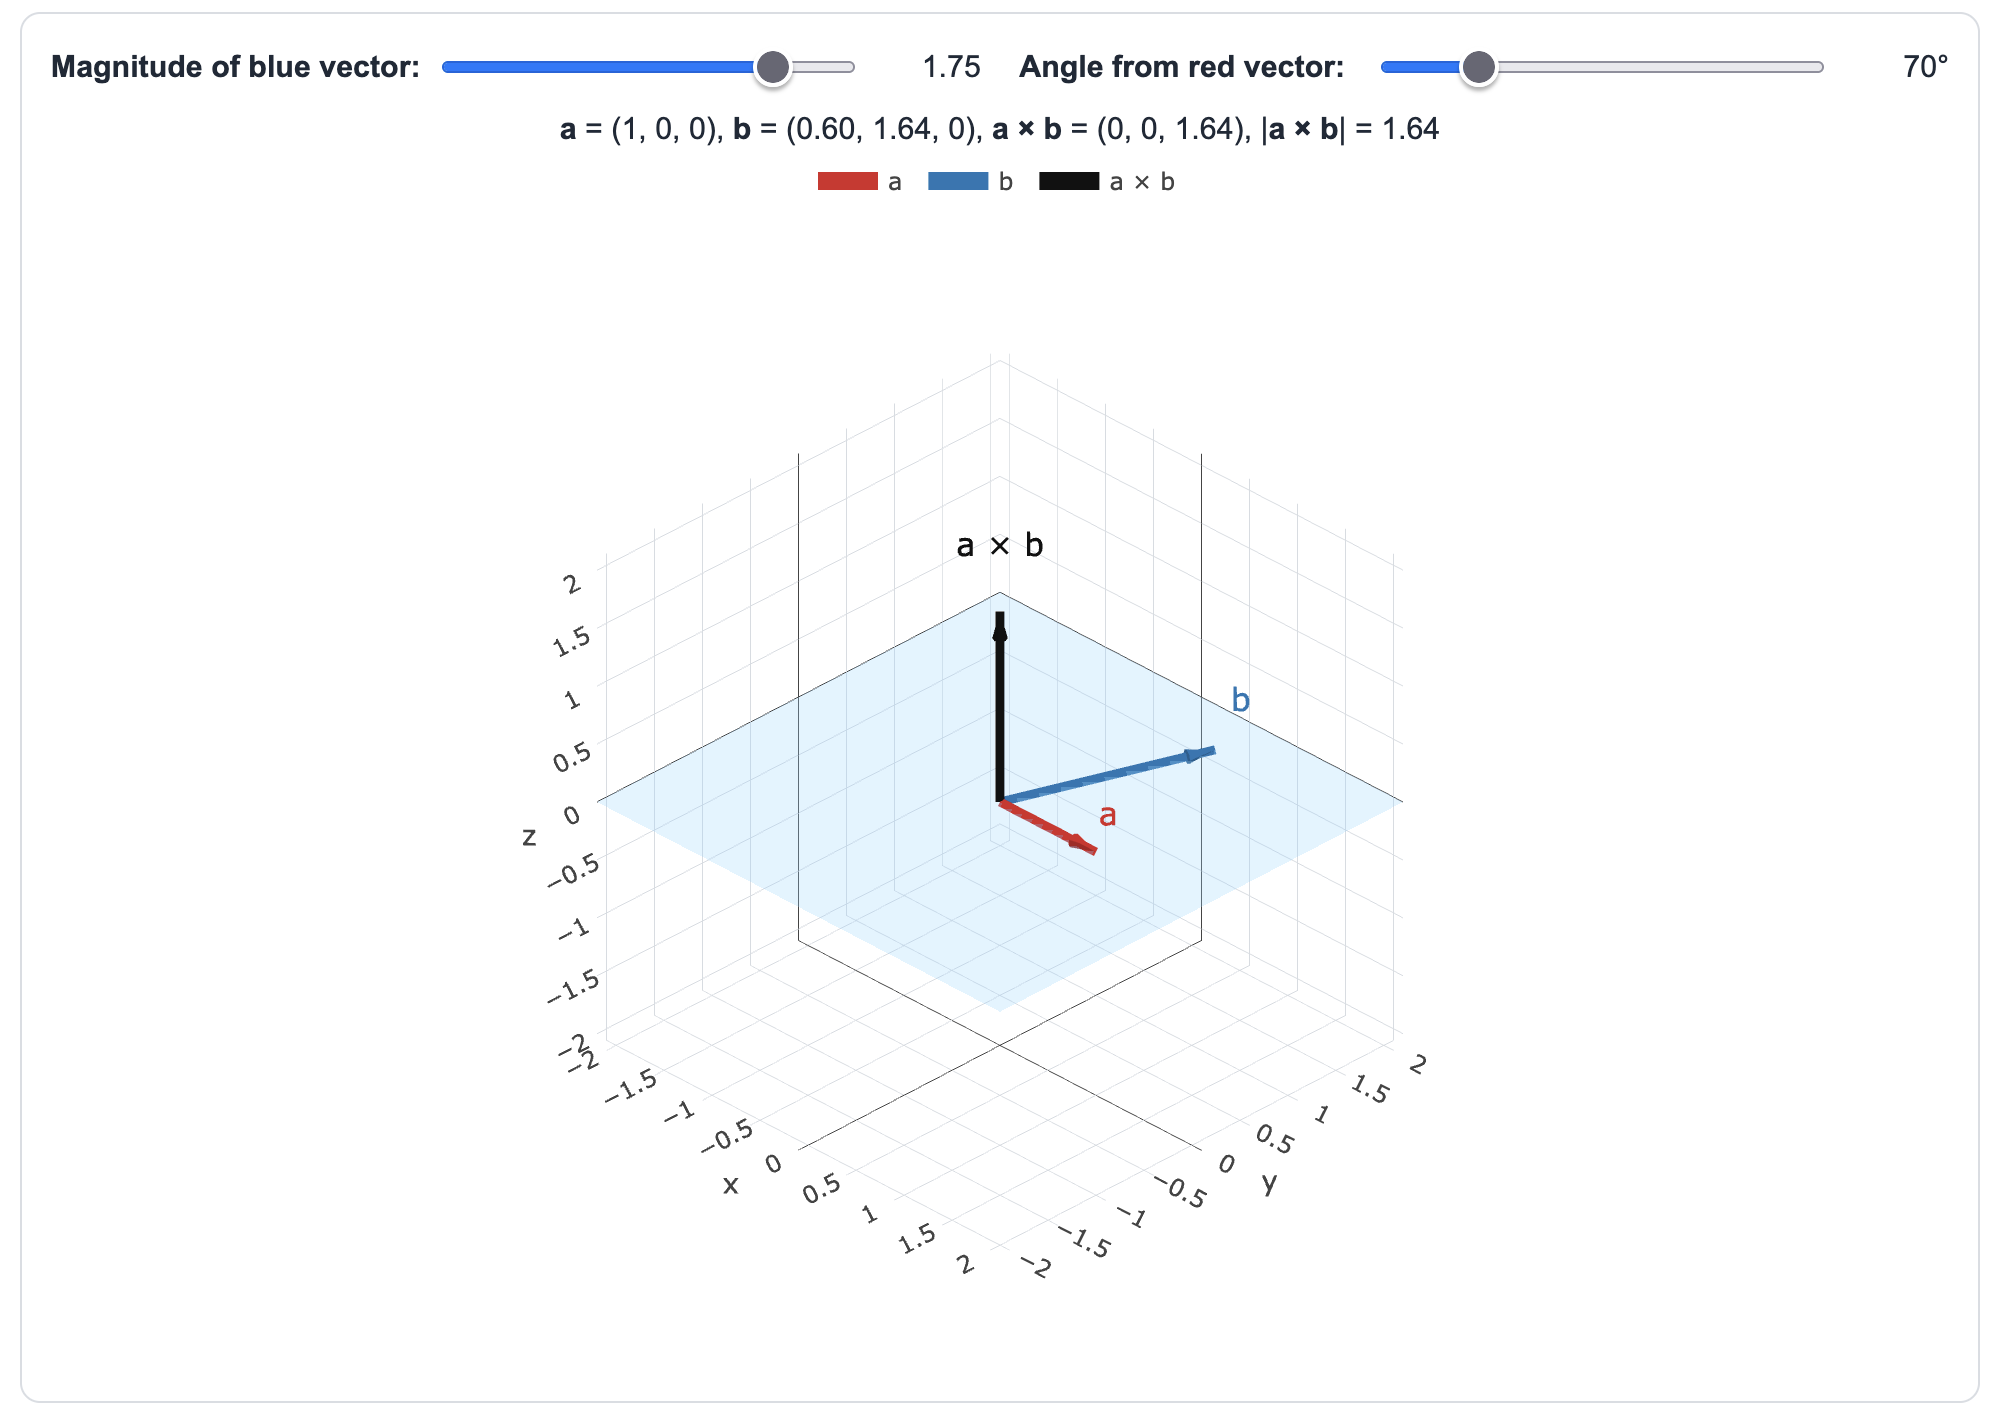
\includegraphics[width=0.9\textwidth]{Figures/Section4/cross_product.png}
    \caption{Screenshots of the interactive plot of the vector product $\myvec{a} \times \myvec{b}$, available in the HTML version of these notes. The black vector show the resulting vector from taking the cross product of the red vector with the blue vector.}
    \fi
    \label{anim:cross_prod}
\end{figure}

\begin{example}[DIY]
A wire carries current $I=1$ [A] along its length, given by the vector
\[
\myvec{l}=0.2\myvec{i}\;[\mathrm{m}].
\]
It is placed in a magnetic field
\[
\myvec{B}=-3\myvec{j}\;[\mathrm{T}].
\]
Calculate the magnetic force acting on the wire, given by
\[
\myvec{F}=I(\myvec{l}\times\myvec{B}).
\]
\begin{center}
    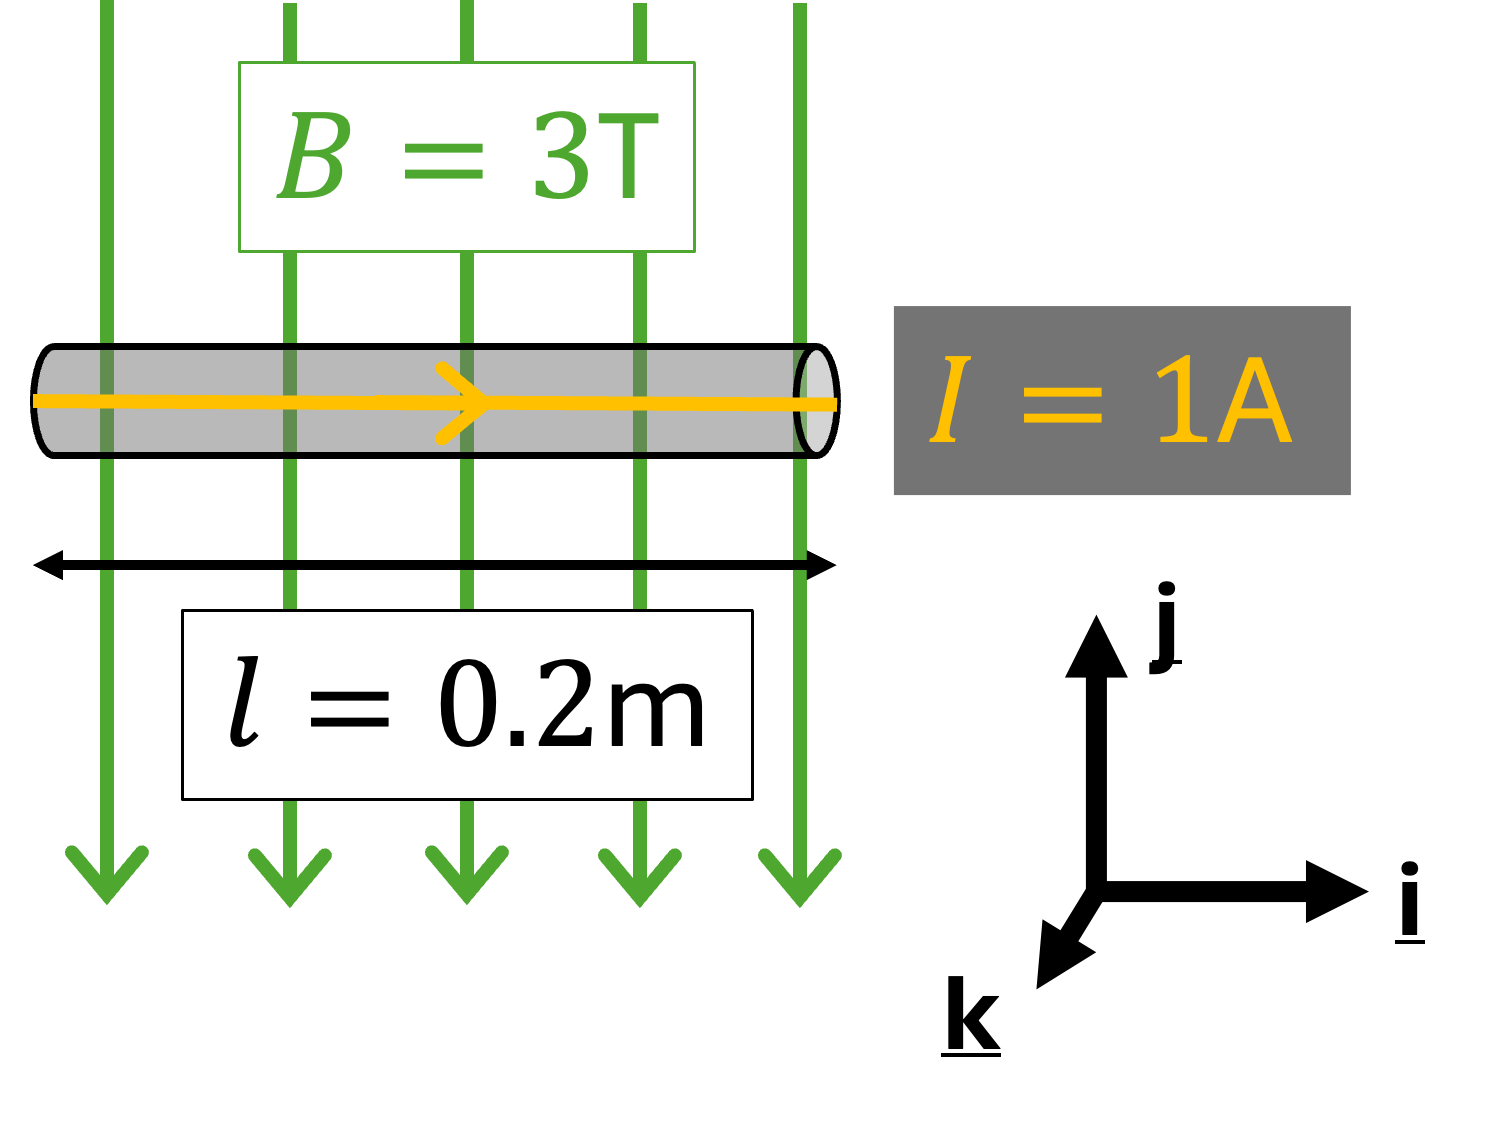
\includegraphics[width=0.4\textwidth]{Figures/Section4/Ex441.png}
\end{center}
\end{example}

\begin{blanksol}
Using the right-hand rule, the direction of $\myvec{l}\times\myvec{B}$ is $-\myvec{k}$.

The magnitude of $\myvec{l}\times\myvec{B}$ is given by
\[
\left\lvert\myvec{l}\times\myvec{B}\right\rvert
=\lvert\myvec{l}\rvert\lvert\myvec{B}\rvert\sin\theta
=0.2\times3\times1=0.6.
\]
And so
\[
\myvec{F}=1\times0.6\times(-\myvec{k})=-0.6\myvec{k}\;[\mathrm{N}].
\]
\end{blanksol}

\textbf{The Vector Product in Component form.} Defining $\myvec{a} = (a_x\myvec{i}+a_y\myvec{j}+a_z\myvec{k})$ and $\myvec{b} = (b_x\myvec{i}+b_y\myvec{j}+b_z\myvec{k})$, the vector product is given by
\begin{align}
    \myvec{a} \times \myvec{b} &= (a_yb_z-a_zb_y)\myvec{i}
    +(a_zb_x-a_xb_z)\myvec{j}
    +(a_xb_y-a_yb_x)\myvec{k}.
\end{align}

This is equivalent to the following determinant
\begin{equation}
    \myvec{a}\times\myvec{b}
=
\begin{vmatrix}
\myvec{i}&\myvec{j}&\myvec{k}\\
a_x&a_y&a_z\\
b_x&b_y&b_z
\end{vmatrix}.
\end{equation}

\begin{example}[Lecture]
If
\[
\myvec{a}=2\myvec{i}-\myvec{j}+3\myvec{k}
\qquad\text{and}\qquad
\myvec{b}=3\myvec{i}+2\myvec{j}-4\myvec{k},
\]
find the vector product $\myvec{a}\times\myvec{b}$.
\end{example}

\begin{solution}
\begin{align*}
    \myvec{a}\times\myvec{b}
    & =\begin{vmatrix}\myvec{i}&\myvec{j}&\myvec{k}\\2&-1&3\\3&2&-4\end{vmatrix}\\
    & =\blank{((-1)(-4)-3\times2)\myvec{i}+(3\times3-2(-4))\myvec{j}+(2\times2-(-1)3)\myvec{k}}\\
 &= \blank{(4-6)\myvec{i}+(9+8)\myvec{j}+(4+3)\myvec{k} = -2\myvec{i}+17\myvec{j}+7\myvec{k}}
\end{align*}

% In determinant form
% \[
% \myvec{a}\times\myvec{b}
% =
% \begin{vmatrix}
% \myvec{i}&\myvec{j}&\myvec{k}\\
% 2&-1&3\\
% 3&2&-4
% \end{vmatrix}
% \]
% \[
% =((-1)(-4)-3\times2)\myvec{i}
% +(3\times3-2(-4))\myvec{j}
% +(2\times2-(-1)3)\myvec{k}
% \]
% \[
% =(4-6)\myvec{i}+(9+8)\myvec{j}+(4+3)\myvec{k}
% =-2\myvec{i}+17\myvec{j}+7\myvec{k}.
% \]
\end{solution}

\textbf{Properties of Vector Products.} The vector product does not commute, in fact it is \textbf{anti-commutative}, so
\begin{equation}
    \myvec{a}\times\myvec{b}=-(\myvec{b}\times\myvec{a}).    
\end{equation}

Multiplying vectors by a scalar only changes their magnitude, not direction, so 
\begin{equation}
    (\alpha\myvec{a})\times\myvec{b}
=\alpha(\myvec{a}\times\myvec{b})
=\myvec{a}\times(\alpha\myvec{b}).
\end{equation}
This follows from the definition $\left\lvert\myvec{a}\times\myvec{b}\right\rvert
=\lvert\myvec{a}\rvert\lvert\myvec{b}\rvert\sin\theta$, since
\[
\lvert\alpha\myvec{a}\rvert\lvert\myvec{b}\rvert\sin\theta
=\alpha\lvert\myvec{a}\rvert\lvert\myvec{b}\rvert\sin\theta
=\lvert\myvec{a}\rvert\lvert\alpha\myvec{b}\rvert\sin\theta. 
\]

\begin{example}[Video]
For the vectors
\[
\myvec{a}=2\myvec{i}-\myvec{j}+3\myvec{k}
\qquad\text{and}\qquad
\myvec{b}=3\myvec{i}+2\myvec{j}-4\myvec{k}
\]
and scalar $\alpha=5$, verify that
\[
(\alpha\myvec{a})\times\myvec{b}
=\myvec{a}\times(\alpha\myvec{b})
=\alpha(\myvec{a}\times\myvec{b}).
\]
\end{example}

\begin{solution}
First calculate 
\begin{align*}
    \alpha\myvec{a} &= 5(2\myvec{i}-\myvec{j} + 3\myvec{k}) = 10\myvec{i} - 5\myvec{j} + 15\myvec{k} \\
    \alpha\myvec{b} &= 5(3\myvec{i} + 2\myvec{j} - 4\myvec{k}) = 15\myvec{i} + 10\myvec{j} - 20\myvec{k}
\end{align*}

Take the first case
\begin{align*}
    (\alpha\myvec{a})\times\myvec{b}
= \begin{vmatrix}\myvec{i}&\myvec{j}&\myvec{k}\\10&-5&15\\3&2&-4\end{vmatrix}
&=\blank{(20-30)\myvec{i}+(45-(-40))\myvec{j}+(20-(-15))\myvec{k}}\\
&=\blank{-10\myvec{i}+85\myvec{j}+35\myvec{k}}
\end{align*}

In the second case
\begin{align*}
\myvec{a}\times(\alpha\myvec{b})
= \begin{vmatrix}\myvec{i}&\myvec{j}&\myvec{k}\\2&-1&3\\15&10&-20\end{vmatrix}
&=\blank{(20-30)\myvec{i}+(45-(-40))\myvec{j}+(20-(-15))\myvec{k}}\\
&= \blank{-10\myvec{i}+85\myvec{j}+35\myvec{k}}
\end{align*}

Finally
\begin{align*}
    \alpha(\myvec{a}\times\myvec{b})
= 5\begin{vmatrix}\myvec{i}&\myvec{j}&\myvec{k}\\2&-1&3\\3&2&-4\end{vmatrix}
&=\blank{5[(4-6)\myvec{i}+(9-(-8))\myvec{j}+(4-(-3))\myvec{k}]}\\
&=\blank{5(-2\myvec{i}+17\myvec{j}+7\myvec{k}) = -10\myvec{i}+85\myvec{j}+35\myvec{k}}
\end{align*}
\end{solution}

The vector product is \textbf{distributive}, \textit{i.e}.
\begin{equation}
    \myvec{a}\times(\myvec{b}+\myvec{c})
=(\myvec{a}\times\myvec{b})+(\myvec{a}\times\myvec{c}).
\end{equation}
And so
\[
\myvec{a}\times(\myvec{b}-\myvec{c})
=(\myvec{a}\times\myvec{b})-(\myvec{a}\times\myvec{c}).
\]

\textbf{Parallel} (and \textbf{anti-parallel}) vectors have a cross product of $\myvec{0}$. A special case of this is
\[
\myvec{a}\times\myvec{a}=\myvec{0}.
\]
Again, this can be seen from the definition $
\left\lvert\myvec{a}\times\myvec{b}\right\rvert
=\lvert\myvec{a}\rvert\lvert\myvec{b}\rvert\sin\theta$,
as the angle $\theta=0$ for parallel vectors and $\theta=\pi$ for anti-parallel vectors.

\textbf{Areas of Parallelograms and Triangles.} Consider the parallelogram with sides given by the vectors $\myvec{a}$ and $\myvec{b}$ in figure \ref{fig:parallelo}(a). The `height' of the parallelogram is given by $\lvert\myvec{b}\rvert\sin\theta$. So, the area is
\[
\lvert\myvec{a}\rvert\lvert\myvec{b}\rvert\sin\theta
=\left\lvert\myvec{a}\times\myvec{b}\right\rvert.
\]

Now, consider the triangle with sides given by the vectors $\myvec{a}$ and $\myvec{b}$ in figure \ref{fig:parallelo}(b). The triangle has half of the area of the parallelogram in figure \ref{fig:parallelo}(a) and so the area is $\frac{1}{2}\left\lvert \myvec{a}\times\myvec{b} \right\rvert$.
\begin{figure}
    \centering
    \subfig{0.46}{Figures/Section4/44d_parallelo.png}{Parallelogram}
    \subfig{0.34}{Figures/Section4/44e_triangle.png}{Triangle}
    \caption{The magntiude of the vector product $\left\lvert\myvec{a}\times\myvec{b}\right\rvert$ gives the area of the parallelogram formed by $\myvec{a}$ and $\myvec{b}$ in (a). Halving this gives the area of the yellow (or orange) triangle in (b).}
    \label{fig:parallelo}
\end{figure}

\begin{example}[Lecture]
Find the area of the triangle with two sides given by the vectors
\[
\myvec{a}=2\myvec{i}-\myvec{j}+3\myvec{k}
\qquad\text{and}\qquad
\myvec{b}=-2\myvec{i}+17\myvec{j}+7\myvec{k}.
\]
\end{example}

\begin{solution}
In determinant form
\begin{align*}
\myvec{a}\times\myvec{b}
&=
\begin{vmatrix}
\myvec{i}&\myvec{j}&\myvec{k}\\
2&-1&3\\
-2&17&7
\end{vmatrix}\\
&=\blank{(-7-51)\myvec{i}+(-6-14)\myvec{j}+(34-2)\myvec{k}}\\
&=\blank{-58\myvec{i}-20\myvec{j}+32\myvec{k}}.
\end{align*}
The area of the triangle is
\begin{align*}
\frac{1}{2}\left\lvert\myvec{a}\times\myvec{b}\right\rvert
&=\blank{\frac{1}{2}\sqrt{(-58)^2+(-20)^2+32^2}}\\
&=\blank{\frac{1}{2}\sqrt{4788} =\sqrt{1197}} \approx \blank{34.6}.
\end{align*}
\end{solution}

\begin{exammistake}
Remember, the result of the \textbf{scalar} product is a \textbf{scalar}, and the result of the \textbf{vector} product is a \textbf{vector}.

\textbf{25/26 In class assessment 2 (discontinued)}

Given that
\[
\myvec{a}=-8\myvec{i}-2\myvec{j}+4\myvec{k}
\]
and that
\[
\myvec{b}=7\myvec{i}-5\myvec{j}+2\myvec{k},
\]
input the scalar or ``dot'' product
\[
\myvec{a}\boldsymbol{\cdot}\myvec{b}= \_\_\_\_.
\]

Several people tried to input a vector, which was not accepted by STACK, causing some confusion and frustration.
\end{exammistake}

\begin{recap}{\ref{sec:cross_prod}}
\item The result of $\myvec{a}\times\myvec{b}$ is a \textbf{vector} perpendicular to $\myvec{a}$ and $\myvec{b}$.
\item The direction of the result can be found by the \textbf{right-hand rule}.
\[
\left\lvert\myvec{a}\times\myvec{b}\right\rvert
=\lvert\myvec{a}\rvert\lvert\myvec{b}\rvert\sin\theta,
\]
which is the \textbf{area} of the relevant parallelogram.
\item It can be calculated using the determinant, or in component form
\[
(a_yb_z-a_zb_y)\myvec{i}
+(a_zb_x-a_xb_z)\myvec{j}
+(a_xb_y-a_yb_x)\myvec{k}.
\]
\item The cross product of a vector with itself is
\[
\myvec{a}\times\myvec{a}=\myvec{0}.
\]
\end{recap}

\subsection{Vectors, lines, and planes}
\label{sec:line_plane}

\begin{learningoutcomes}
\item Write the vector equations for a line and a plane
\item Find crossing points of lines and planes given in vector form
\end{learningoutcomes}

\textbf{Vectors and Lines.} A line passing through point $A$ (with position vector $\myvec{a}$) and parallel to vector $\myvec{b}$ has equation
\begin{equation}
    \label{eq:vecline} \myvec{r}=\myvec{a}+\lambda\myvec{b}.
\end{equation}
Here, $\lambda$ is a parameter and every value of $\lambda$ represents a different point on the line (see figure \ref{fig:vecline}.
\begin{figure}
    \centering
    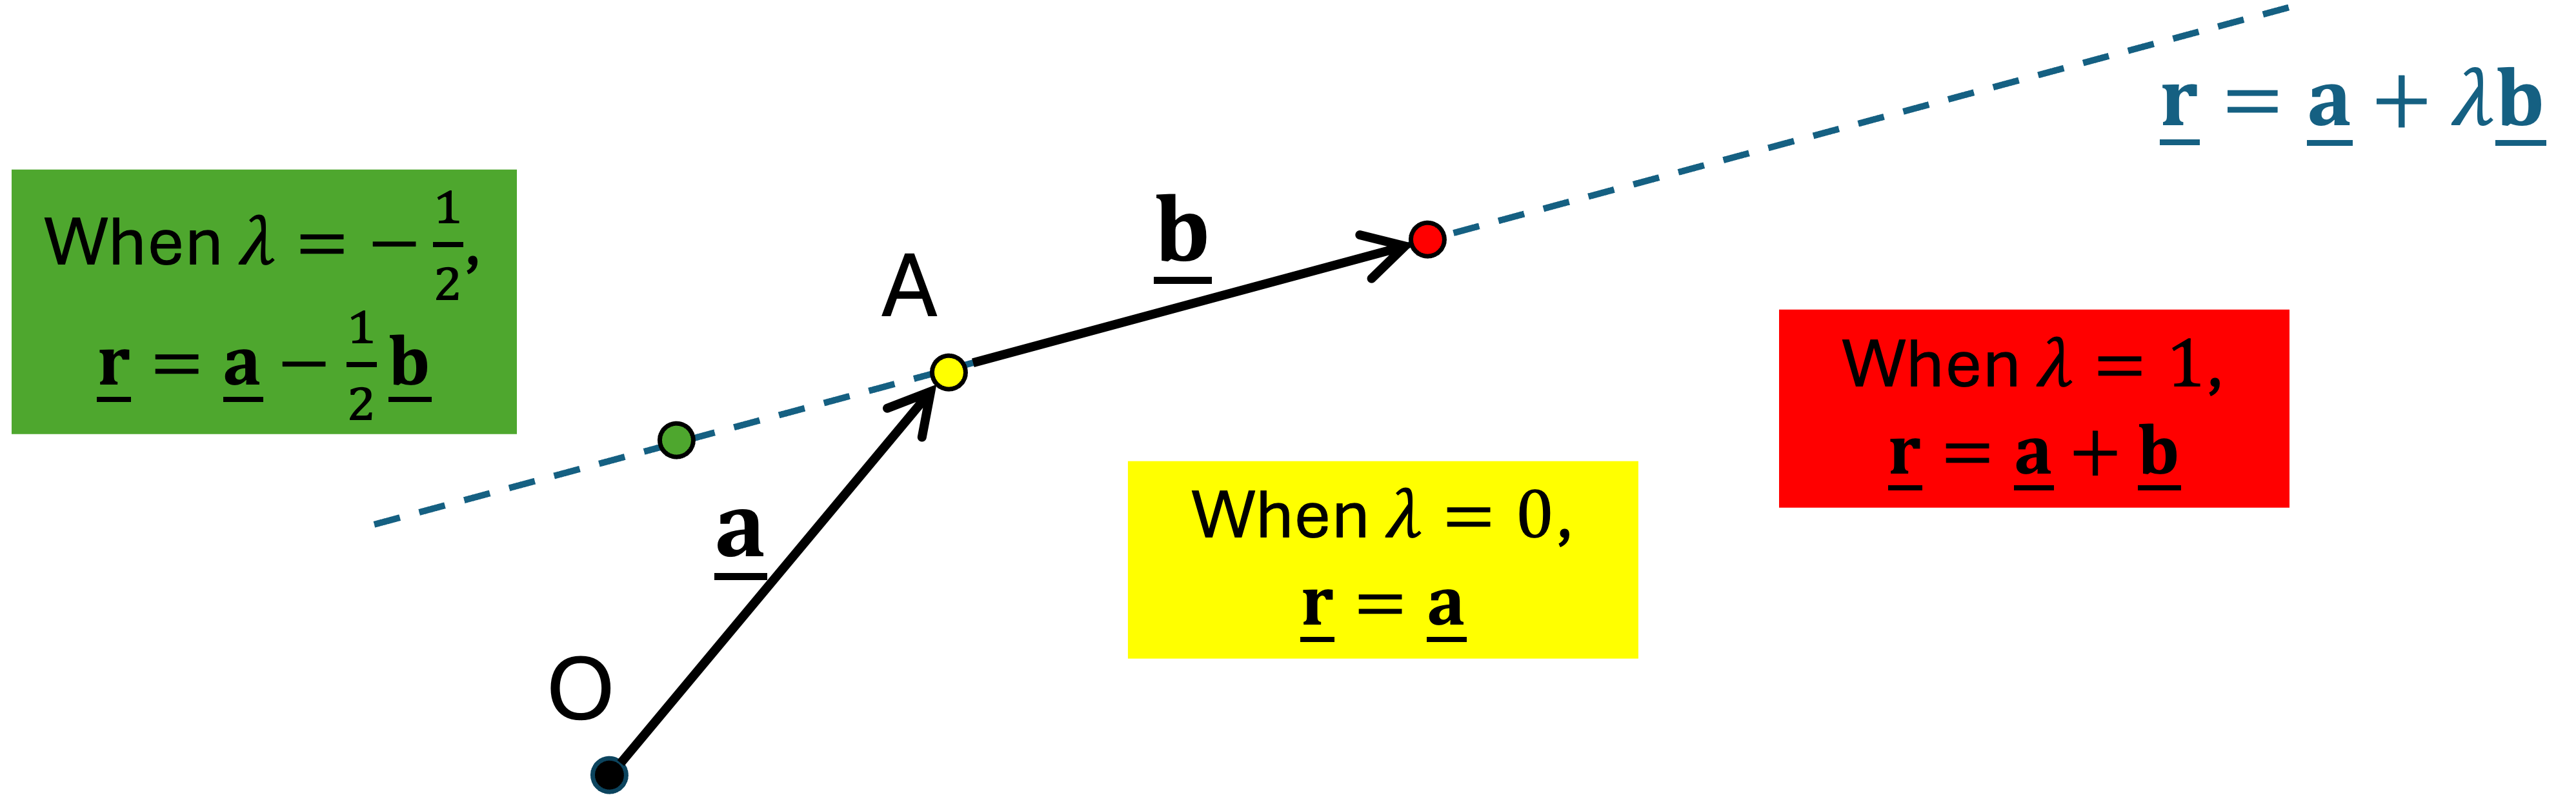
\includegraphics[width=0.8\linewidth]{Figures/Section4/45a_line_eq.png}
    \caption{Illustration of points on the line given by different values of the parameter $\lambda$ in equation \eqref{eq:vecline}.}
    \label{fig:vecline}
\end{figure}

To find a line passing through points with position vectors $\myvec{p}$ and $\myvec{q}$:
\begin{itemize}
\item Choose $\lambda=0$ for when $\myvec{r}=\myvec{p}$, \emph{i.e.} set $\myvec{a}=\myvec{p}$.
\item Choose $\lambda=1$ for when $\myvec{r}=\myvec{q}$, \emph{i.e.} set $\myvec{b}=\myvec{q}-\myvec{p}$.
\end{itemize}
Therefore, the equation becomes
\[
\myvec{r}=\myvec{p}+\lambda(\myvec{q}-\myvec{p}).
\]

\begin{example}[Lecture]
(a) Find the vector equation of the line through the two points $(2,1,5)$ and $(4,3,-2)$.

(b) By eliminating any parameter, write this in the form
\[
\frac{x-x_0}{a}=\frac{y-y_0}{b}=\frac{z-z_0}{c}.
\]
\end{example}

\begin{solution}
Define
\[
\myvec{p}=\begin{pmatrix}2\\1\\5\end{pmatrix}
\qquad\text{and}\qquad
\myvec{q}=\begin{pmatrix}4\\3\\-2\end{pmatrix}.
\]
Then the equation of the line is
\begin{align*}
    \myvec{r}&= \blank{\myvec{p}+\lambda(\myvec{q}-\myvec{p})} \\
             &= \begin{pmatrix}2\\1\\5\end{pmatrix}
 + \lambda\begin{pmatrix}2\\2\\-7\end{pmatrix}.
\end{align*}

(b) Writing
\[
\myvec{r}=\begin{pmatrix}x\\y\\z\end{pmatrix}
\]
gives equations for $x$, $y$, and $z$ in terms of $\lambda$:
\[
x=\blank{2+2\lambda},
\qquad
y=\blank{1+2\lambda},
\qquad
z=\blank{5-7\lambda}.
\]
Each of these can be rearranged in terms of $\lambda$:
\[
\lambda= \blank{\frac{x-2}{2}},
\qquad
\lambda= \blank{\frac{y-1}{2}},
\qquad
\lambda= \blank{\frac{z-5}{-7}}.
\]
All of these expressions must be equal, so
\[
\blank{\frac{x-2}{2}=\frac{y-1}{2}=\frac{z-5}{-7}}.
\]
Comparing to the original expression:
\[
x_0= \blank{2},
\qquad a= \blank{2},
\qquad y_0= \blank{1},
\qquad b= \blank{2},
\qquad z_0= \blank{5},
\qquad c= \blank{-7}.
\]
\end{solution}

To find whether the lines
\[
\myvec{r}_1=\myvec{a}+\lambda\myvec{b} \qquad \mathrm{and} \qquad 
\myvec{r}_2=\myvec{c}+\mu\myvec{d}
\]
cross, we need to equate $\myvec{r}_1=\myvec{r}_2$. \emph{I.e.} it is necessary to find values of $\lambda$ and $\mu$ that satisfy \textbf{all} components. If the lines do not cross, this will not be possible.
\begin{itemize}
\item In 2D, lines that do not cross are parallel, which would mean here that $\myvec{b}$ was parallel (or anti-parallel) to $\myvec{d}$ (see figure \ref{fig:twoveclines}).
\item In 3D, two lines do not cross in general.
\end{itemize}
\begin{figure}
    \centering
    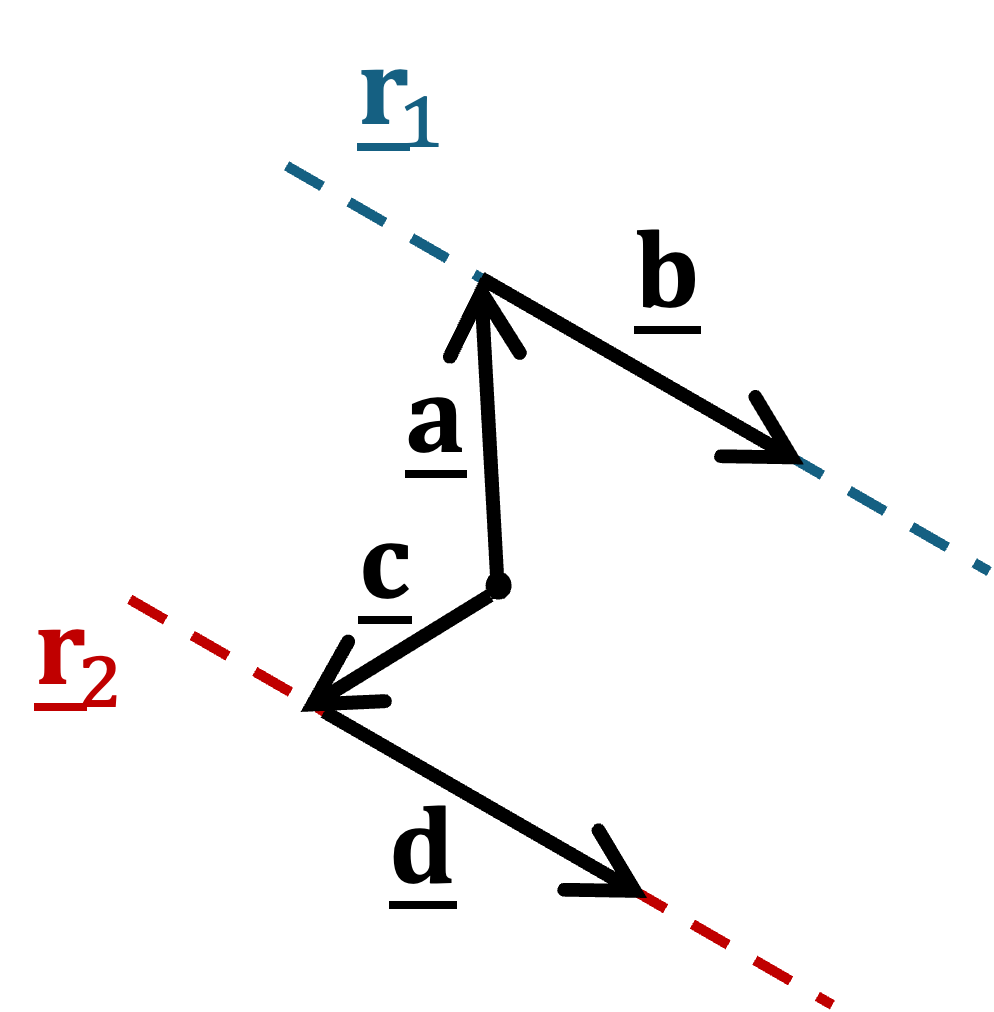
\includegraphics[width=0.25\linewidth]{Figures/Section4/45b_parallel.png}
    \caption{A sketch of when the lines $\myvec{r}_1=\myvec{a}+\lambda\myvec{b}$ and $\myvec{r}_2=\myvec{c}+\mu\myvec{d}$ are parallel.}
    \label{fig:twoveclines}
\end{figure}

\begin{example}[Lecture]
There is one value of $w$ for which the lines
\[
\myvec{r}_1=\begin{pmatrix}2\\-1\\4\end{pmatrix}
+\lambda\begin{pmatrix}1\\2\\-1\end{pmatrix}
\]
and
\[
\myvec{r}_2=\begin{pmatrix}5\\2\\w\end{pmatrix}
+\mu\begin{pmatrix}1\\-1\\-3\end{pmatrix}
\]
cross. Find this value of $w$ and the crossing point.
\end{example}

\begin{solution}
Start by setting the lines equal $\myvec{r}_1=\myvec{r}_2$ and so the $x$- and $y$- components are
\begin{align*}
    \blank{2+\lambda} &= \blank{5+\mu,}
    \blank{-1+2\lambda} &= \blank{2-\mu.}
\end{align*}
Adding these two equations together gives 
\[
\blank{1 + 3\lambda = 7}
\]
and so $\lambda=\blank{2}$ and therefore $\mu=\blank{-1}$. Using these values, the $z$-component becomes
\[
\blank{4-2=w+3.}
\]
Therefore, the lines cross when $w=-1$

Substitute the values in to find the crossing point, \textit{e.g.} using $\lambda=\blank{2}$ in $\myvec{r}_1$ gives
\[
\myvec{r}_1
=\blank{\begin{pmatrix}2 + 2\\-1 + 4\\4 - 2\end{pmatrix}
=\begin{pmatrix}4\\3\\2\end{pmatrix}}
\]
\end{solution}

\textbf{Vector equation of a plane.} A plane can be uniquely specified by
\begin{itemize}
\item A point on the plane, $A$ (with position vector $\myvec{a}$).
\item \textbf{and} a vector perpendicular to the plane, $\myvec{n}$.
\end{itemize}

If the point $P$ (with position vector $\myvec{r}$) is also on the plane then $\overrightarrow{AP}$ must lie in the plane, and so $\overrightarrow{AP}$ is perpendicular to $\myvec{n}$ (figure \ref{fig:plane}(a)). Since $\overrightarrow{AP}=\myvec{r}-\myvec{a}$ is perpendicular to $\myvec{n}$, then $(\myvec{r}-\myvec{a})\boldsymbol{\cdot}\myvec{n}=0$, and so, by the distributive property,
\[
\myvec{r}\boldsymbol{\cdot}\myvec{n}
=\myvec{a}\boldsymbol{\cdot}\myvec{n}.
\]
This is the vector equation of a plane.

Defining
\[
\myvec{r}=\begin{pmatrix}x\\y\\z\end{pmatrix},
\qquad
\myvec{n}=\begin{pmatrix}a\\b\\c\end{pmatrix},
\qquad
\myvec{a}\boldsymbol{\cdot}\myvec{n}=d,
\]
we return to the algebraic form for the equation of a plane
\[
ax+by+cz=d.
\]
Note, often the unit normal vector $\hat{\myvec{n}}$ is used, so the equation of the plane becomes $\myvec{r}\boldsymbol{\cdot}\hat{\myvec{n}}
=\myvec{a}\boldsymbol{\cdot}\hat{\myvec{n}}$.

An equivalent way to represent the equation of a plane is
\[
\myvec{r}\boldsymbol{\cdot}\hat{\myvec{n}}=d,
\]
The geometric interpretation of this is that all points on the plane are the same perpendicular distance $d$ from the origin, as sketched in figure \ref{fig:plane}(b).
\begin{figure}
    \centering
    \subfig{0.4}{Figures/Section4/45c_plane1.png}{Looking down}
    \subfig{0.4}{Figures/Section4/45d_plane2.png}{Side view}
    \caption{Sketches of the definition of the plane defined by the point $A$ and normal vector $\myvec{n}$. The equation $\myvec{r}\boldsymbol{\cdot}\hat{\myvec{n}}
=\myvec{a}\boldsymbol{\cdot}\hat{\myvec{n}}$ is satisfied for a position vector $\myvec{r}$ that points to some point $P$ on the plane. }
    \label{fig:plane}
\end{figure}

\begin{example}[Lecture]
Write the vector equation of the plane that contains the points
\[
A=(0,2,-2),
\qquad
B=(6,2,0),
\qquad
C=(3,5,1).
\]
\end{example}

\begin{solution}
$\overrightarrow{AB}$ and $\overrightarrow{AC}$ lie in the plane, therefore $\overrightarrow{AB}\times\overrightarrow{AC}$ is perpendicular to the plane
\[
\overrightarrow{AB}=\blank{\begin{pmatrix}6\\2\\0\end{pmatrix}-\begin{pmatrix}0\\2\\-2\end{pmatrix}=\begin{pmatrix}6\\0\\2\end{pmatrix}},
\qquad
\overrightarrow{AC}=\blank{\begin{pmatrix}3\\5\\1\end{pmatrix}-\begin{pmatrix}0\\2\\-2\end{pmatrix}=\begin{pmatrix}3\\3\\3\end{pmatrix}}
\]
\begin{align*}
\overrightarrow{AB}\times\overrightarrow{AC}
&=\begin{vmatrix}\myvec{i}&\myvec{j}&\myvec{k}\\\blank{6}&\blank{0}&\blank{2}\\\blank{3}&\blank{3}&\blank{3}\end{vmatrix}\\
&=\blank{-6\myvec{i}+(6-18)\myvec{j}+18\myvec{k}=\begin{pmatrix}-6\\-12\\18\end{pmatrix}}\\
&=\blank{\begin{pmatrix}-6\\-12\\18\end{pmatrix}}
\end{align*}
Choose $\myvec{n}=\blank{-\frac{1}{6}(\overrightarrow{AB}\times\overrightarrow{AC})=\myvec{i}+2\myvec{j}-3\myvec{k}}$
and $\myvec{a}=\blank{2\myvec{j}-2\myvec{k}}$ then
\[
\myvec{a}\cdot\myvec{n}= \blank{4+6=10}
\]
and so the equation of the plane is
\[
\blank{\myvec{r}\cdot\begin{pmatrix}1\\2\\-3\end{pmatrix}}=\blank{10}
\]
\end{solution}

\begin{example}[Video]
Find where the line
\[
\myvec{r}_1
=\begin{pmatrix}1\\-2\\0\end{pmatrix}
+\lambda\begin{pmatrix}3\\1\\-1\end{pmatrix}
\]
intersects the plane
\[
\myvec{r}\boldsymbol{\cdot}
\begin{pmatrix}1\\0\\1\end{pmatrix}=5.
\]
\end{example}

\begin{solution}
Substitute $\myvec{r}=\begin{pmatrix}1\\-2\\0\end{pmatrix}+\lambda\begin{pmatrix}3\\1\\-1\end{pmatrix}$ into the equation for the plane
\[
\blank{\begin{pmatrix}1\\-2\\0\end{pmatrix}\cdot\begin{pmatrix}1\\0\\1\end{pmatrix}
+\lambda\begin{pmatrix}3\\1\\-1\end{pmatrix}\cdot\begin{pmatrix}1\\0\\1\end{pmatrix}=5}
\]
and so
\[
\qquad \blank{1+2\lambda}=5
\]
which gives $\lambda=2$. The intersection point is found by substituting back into $\myvec{r}_1$
\begin{align*}
    \myvec{r}_1(\lambda = \blank{2}) &= 
\blank{\begin{pmatrix}1\\-2\\0\end{pmatrix}+2\begin{pmatrix}3\\1\\-1\end{pmatrix}}\\
&=\blank{\begin{pmatrix}7\\0\\-2\end{pmatrix}=7\myvec{i}-2\myvec{k}}
\end{align*}
\end{solution}

\begin{recap}{\ref{sec:line_plane}}
\item The vector equation of a line is
\[
\myvec{r}=\myvec{a}+\lambda\myvec{b},
\]
where $\myvec{a}$ is the position vector of a point on the line, $\myvec{b}$ gives its direction, and $\lambda$ is a parameter.
\item A line passing through points $\myvec{p}$ and $\myvec{q}$ is
\[
\myvec{r}=\myvec{p}+\lambda(\myvec{q}-\myvec{p}).
\]
\item The vector equation of a plane is
\[
\myvec{r}\boldsymbol{\cdot}\myvec{n}
=\myvec{a}\boldsymbol{\cdot}\myvec{n},
\]
where $\myvec{a}$ is the position vector of a point on the plane, and $\myvec{n}$ is normal to the plane.
\item Crossing points of lines and planes can be found by equating the expressions for $\myvec{r}$.
\end{recap}

\subsection{Triple products}
\label{sec:triple_prod}

\subsubsection{The scalar triple product}

\begin{learningoutcomes}
\item Calculate the different products of three vectors
\item Find the volume of a parallelepiped based on the vectors of three edges
\end{learningoutcomes}

The result of the vector product, \emph{e.g.} $\myvec{b}\times\myvec{c}$, is also a vector. Therefore, scalar and vector products can be applied to it.

When the scalar product is applied, the result is called the scalar triple product
\[
\myvec{a}\boldsymbol{\cdot}(\myvec{b}\times\myvec{c}).
\]

Two equivalent ways to calculate $\myvec{a}\boldsymbol{\cdot}(\myvec{b}\times\myvec{c})$ are:
\begin{itemize}
\item Evaluate $\myvec{b}\times\myvec{c}$ then take the scalar product with $\myvec{a}$.
\item Evaluate the determinant
\begin{equation}
    \myvec{a}\boldsymbol{\cdot}(\myvec{b}\times\myvec{c})
    =
    \begin{vmatrix}
    a_x&a_y&a_z\\
    b_x&b_y&b_z\\
    c_x&c_y&c_z
    \end{vmatrix}.    
\end{equation}
\end{itemize}

\begin{example}[Lecture]
If
\[
\myvec{a}=2\myvec{i}+2\myvec{j}-\myvec{k},
\qquad
\myvec{b}=-\myvec{i}+5\myvec{k},
\qquad
\myvec{c}=6\myvec{i}-\myvec{j},
\]
find $\myvec{a}\boldsymbol{\cdot}(\myvec{b}\times\myvec{c})$:
\begin{itemize}
\item By finding $\myvec{b}\times\myvec{c}$ as an intermediate stage
\item Using the determinant method
\end{itemize}
\end{example}

\begin{solution}
a)
\[
\myvec{b}\times\myvec{c}
=\begin{vmatrix}\myvec{i}&\myvec{j}&\myvec{k}\\-1&0&5\\6&-1&0\end{vmatrix}
=\blank{(0-(-5))\myvec{i}+(30-0)\myvec{j}+(1-0)\myvec{k}=5\myvec{i}+30\myvec{j}+\myvec{k}}
\]
Therefore
\[
\myvec{a}\cdot(\myvec{b}\times\myvec{c})
=\blank{(2\myvec{i}+2\myvec{j}-\myvec{k})\cdot(5\myvec{i}+30\myvec{j}+\myvec{k})=10+60-1=69}
\]
\begin{align*}
    \myvec{a}\cdot(\myvec{b}\times\myvec{c})
&=\begin{vmatrix}2&2&-1\\-1&0&5\\6&-1&0\end{vmatrix}\\
&=\blank{2(0-(-5))+2(30-0)-1(1-0)=10+60-1=69}
\end{align*}
\end{solution}

\textbf{Volume of Parallelepiped.} A parallelepiped is a solid shape with six faces that are parallelogram. If we define the vectors along the edges as $\myvec{a}$, $\myvec{b}$, and $\myvec{c}$, as shown in figure \ref{fig:parallelepiped}, then the area of the base is
\[
\left\lvert\myvec{b}\times\myvec{c}\right\rvert.
\]
The height is $\lvert\myvec{a}\rvert\cos\theta$, where $\theta$ is the angle between $\myvec{a}$ and $\myvec{b}\times\myvec{c}$. So, the volume is
\begin{equation}
    \lvert\myvec{a}\rvert
    \left\lvert\myvec{b}\times\myvec{c}\right\rvert
    \left\lvert\cos\theta\right\rvert
    =
    \left\lvert\myvec{a}\boldsymbol{\cdot}(\myvec{b}\times\myvec{c})\right\rvert.
\end{equation}
\begin{figure}
    \centering
    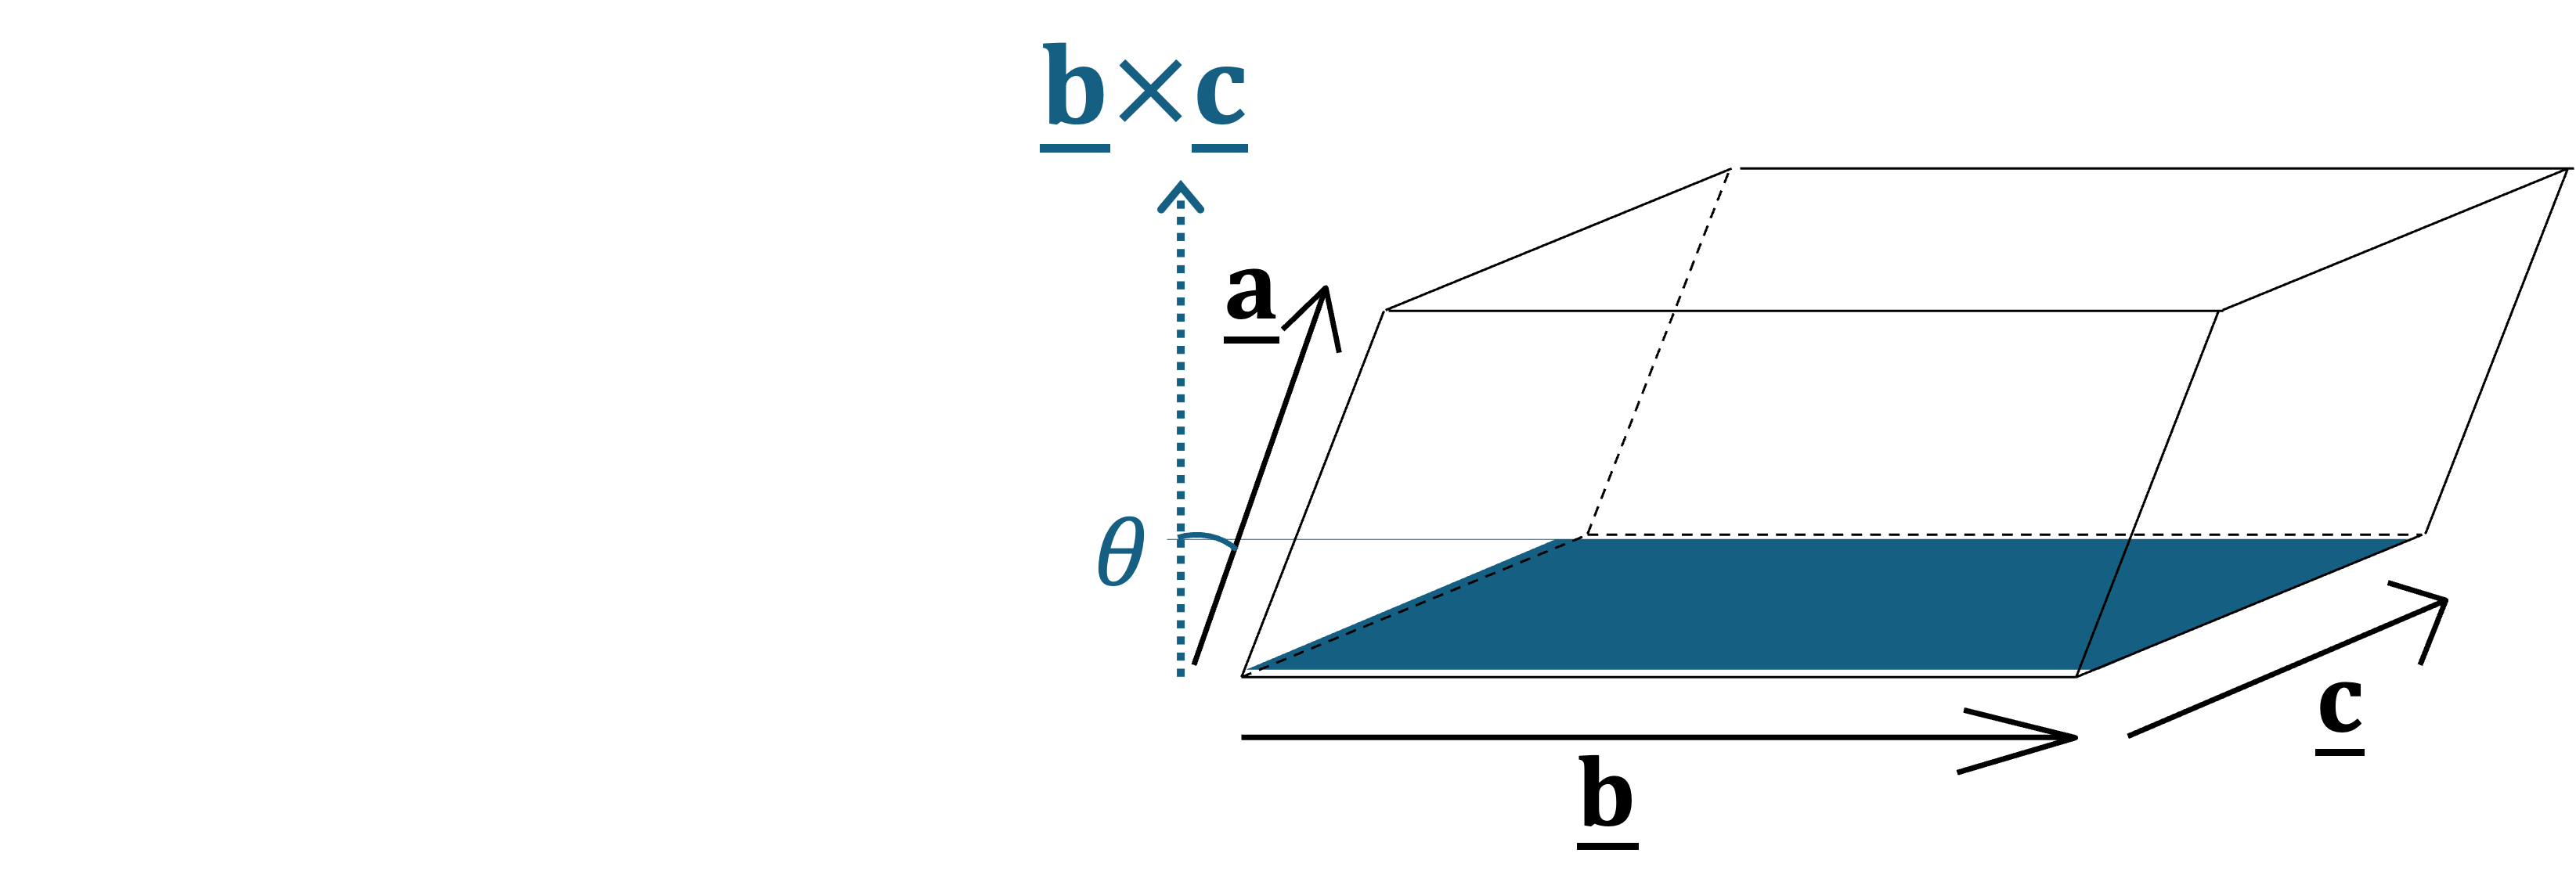
\includegraphics[width=0.7\linewidth]{Figures/Section4/46a_parallelepiped.png}
    \hspace{30mm}
    \caption{Sketch of the parallelepiped defined by the vectors $\myvec{a}$, $\myvec{b}$, and $\myvec{c}$.}
    \label{fig:parallelepiped}
\end{figure}

\begin{example}[Video]
The primitive unit cell of tungsten (shown in orange below) is defined by the vectors
\[
\myvec{u}=\frac{a}{2}(-\myvec{i}+\myvec{j}+\myvec{k}),
\]
\[
\myvec{v}=\frac{a}{2}(\myvec{i}-\myvec{j}+\myvec{k}),
\]
\[
\myvec{w}=\frac{a}{2}(\myvec{i}+\myvec{j}-\myvec{k}),
\]
where $a\approx3.17\,[\text{\AA}]$. Calculate the volume of the primitive unit cell to 3 significant figures. Is there an equivalent primitive unit cell that makes the calculation easier?
\begin{center}
    \iflatexml
        \<div id="bcc-animation">\</div>
        \<script src="bcc-animation.js">\</script>
    \else
        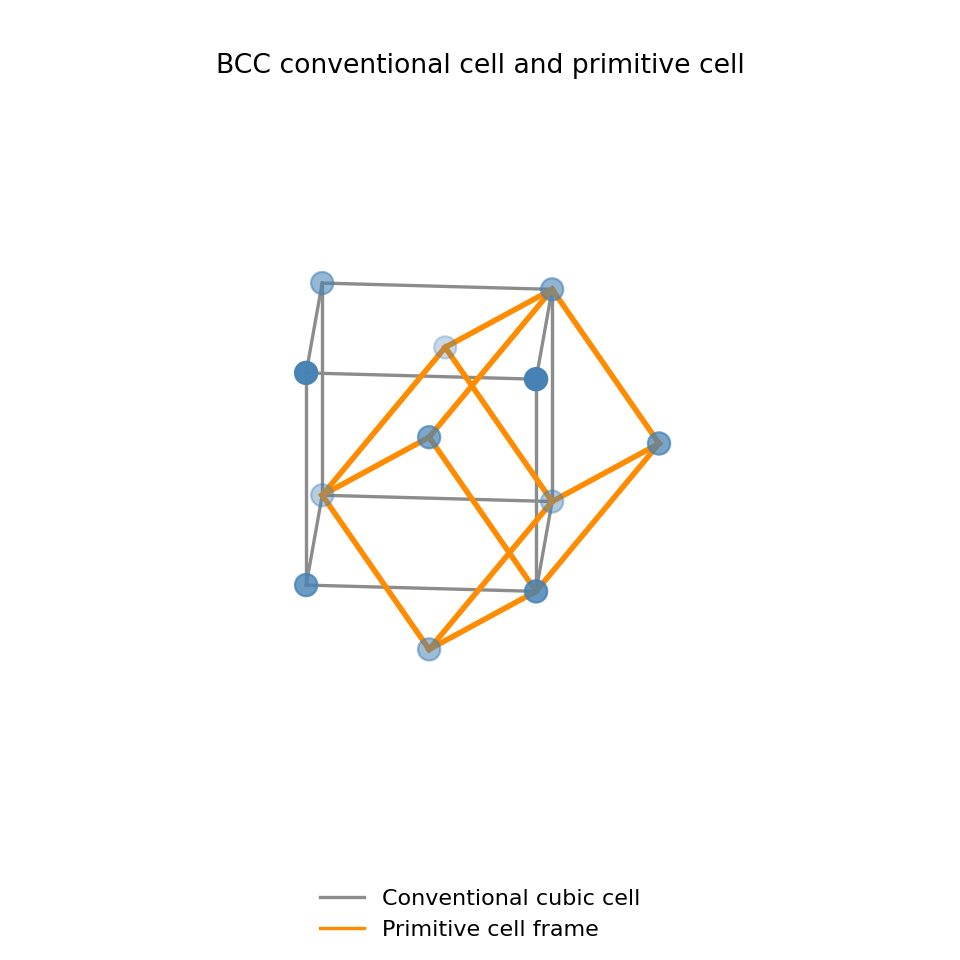
\includegraphics[width=0.6\textwidth]{Figures/Section4/Ex462_bcc.png}
    \fi
\end{center}
\end{example}

\begin{solution}
\begin{align*}
\myvec{u}\boldsymbol{\cdot}(\myvec{v}\times\myvec{w})
&=
\blank{\frac{a^3}{8}
\begin{vmatrix}
-1&1&1\\
1&-1&1\\
1&1&-1
\end{vmatrix}}\\
&=\blank{\frac{a^3}{8}(-1+1+1+1+1+1)
=\frac{a^3}{2}}\\
&\blank{\approx15.9\;[\text{\AA}^3].}
\end{align*}

We could also choose the primitive unit cell defined by
\[
\myvec{u}=\blank{a\myvec{i}},
\qquad
\myvec{v}=\blank{a\myvec{j}},
\qquad
\myvec{w}=\blank{\frac{a}{2}(\myvec{i}+\myvec{j}+\myvec{k})},
\]
which has the same volume, see the figure below for a sketch of this.
\begin{center}
    \iflatexml
        \<div id="bcc-animation-alt">\</div>
        \<script src="bcc-animation-alt.js">\</script>
    \else
        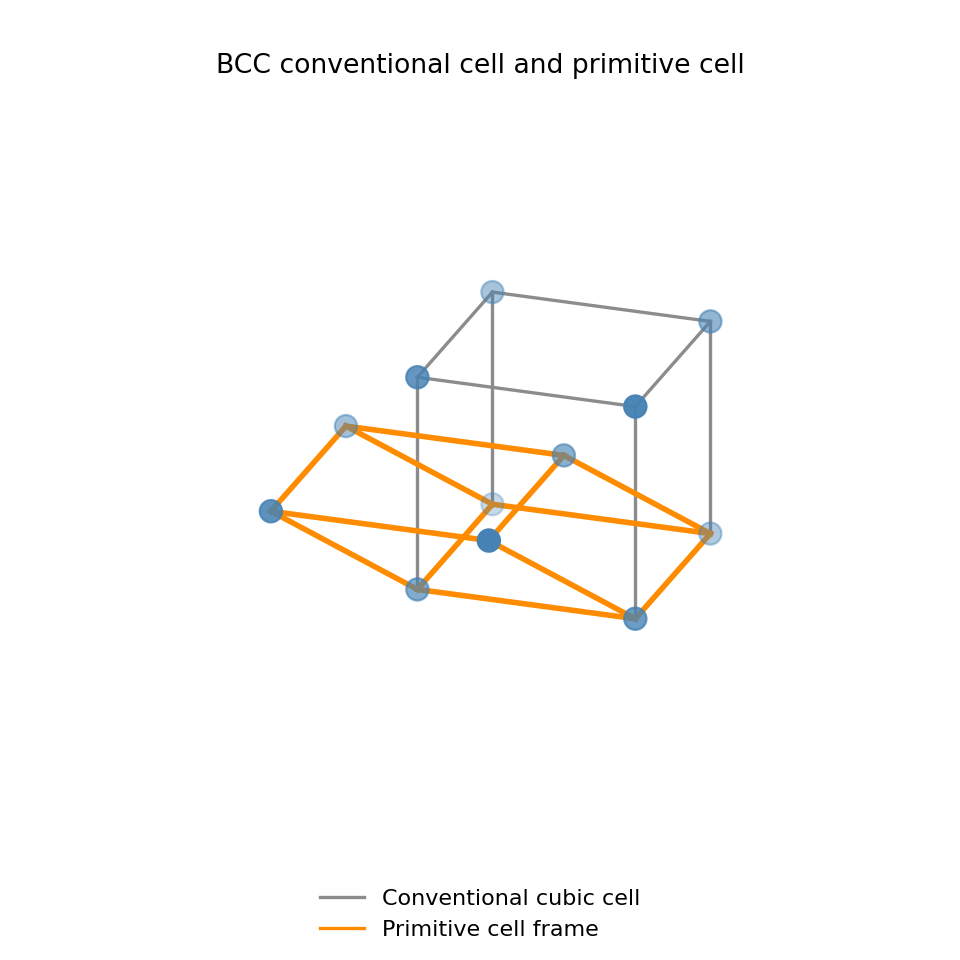
\includegraphics[width=0.6\textwidth]{Figures/Section4/Ex462_bcc_alt.png}
    \fi
\end{center}
\end{solution}

\textbf{Properties of the scalar triple product.} Note that $\myvec{a}\boldsymbol{\cdot}(\myvec{b}\times\myvec{c})
=(\myvec{a}\times\myvec{b})\boldsymbol{\cdot}\myvec{c}$.
Both can be denoted as $[\myvec{a},\myvec{b},\myvec{c}]$

The order of vectors can be cycled without changing the result
\begin{equation}
    [\myvec{a},\myvec{b},\myvec{c}]
=[\myvec{c},\myvec{a},\myvec{b}]
=[\myvec{b},\myvec{c},\myvec{a}].
\end{equation}
Changing the order changes the sign
\begin{equation}
    [\myvec{a},\myvec{c},\myvec{b}]
=[\myvec{b},\myvec{a},\myvec{c}]
=[\myvec{c},\myvec{b},\myvec{a}]
=-[\myvec{a},\myvec{b},\myvec{c}].
\end{equation}

\begin{example}[DIY]
Show that
\[
[\myvec{a},\myvec{a},\myvec{b}]=0
\]
for any $\myvec{a}$ and $\myvec{b}$.
\end{example}

\begin{blanksol}
\[
[\myvec{a},\myvec{a},\myvec{b}]
=\myvec{a}\boldsymbol{\cdot}(\myvec{a}\times\myvec{b}).
\]

$\myvec{v}=\myvec{a}\times\myvec{b}$ is perpendicular to $\myvec{a}$ (i.e. angle between is $\theta=\pi/2$), therefore
\[
\myvec{a}\boldsymbol{\cdot}\myvec{v}
=\lvert\myvec{a}\rvert\lvert\myvec{v}\rvert\cos\theta=0.
\]

Alternatively, by the cyclic property
\[
\myvec{a}\boldsymbol{\cdot}(\myvec{a}\times\myvec{b})
=\myvec{b}\boldsymbol{\cdot}(\myvec{a}\times\myvec{a})=0
\]
since
\[
\myvec{a}\times\myvec{a}=\myvec{0}.
\]
\end{blanksol}

A scalar triple product of zero implies that the three vectors are coplanar \emph{i.e.} in the same plane. It follows that if any two vectors in the product are the same, then the scalar triple product is zero. For example,
\begin{equation}
    [\myvec{a},\myvec{b},\myvec{b}]=0.
\end{equation}

\subsubsection{The vector triple product}

Applying the vector product to a vector product gives the vector triple product
\[
\myvec{a}\times(\myvec{b}\times\myvec{c}).
\]
A useful result i
\begin{equation}
\label{eq:tripcross}
    \myvec{a}\times(\myvec{b}\times\myvec{c})
=(\myvec{a}\boldsymbol{\cdot}\myvec{c})\myvec{b}
-(\myvec{a}\boldsymbol{\cdot}\myvec{b})\myvec{c}.
\end{equation}
Also, note the placement of the parentheses matters
\begin{equation}
\label{eq:tripcross2}
(\myvec{a}\times\myvec{b})\times\myvec{c}
=(\myvec{a}\boldsymbol{\cdot}\myvec{c})\myvec{b}
-(\myvec{b}\boldsymbol{\cdot}\myvec{c})\myvec{a}.
\end{equation}

\begin{example}[Lecture]
Calculate the vector triple product
\[
(\myvec{a}\times\myvec{b})\times\myvec{c},
\]
where
\[
\myvec{a}=2\myvec{i}+2\myvec{j}-\myvec{k},
\]
\[
\myvec{b}=-\myvec{i}+5\myvec{k},
\]
\[
\myvec{c}=6\myvec{i}-\myvec{j}.
\]
\end{example}

\begin{solution}
Use the identity in equation \eqref{eq:tripcross2}
\[
(\myvec{a}\times\myvec{b})\times\myvec{c}
=(\myvec{a}\boldsymbol{\cdot}\myvec{c})\myvec{b}
-(\myvec{b}\boldsymbol{\cdot}\myvec{c})\myvec{a}.
\]
Calculate the scalar products
\begin{align*}
\myvec{a}\boldsymbol{\cdot}\myvec{c}
&=\blank{2\times6+(2\times-1)+(-1\times0)=10},\\
\myvec{b}\boldsymbol{\cdot}\myvec{c}
&=\blank{-1\times6+0\times-1+5\times0=-6}.
\end{align*}

So,
\begin{align*}
(\myvec{a}\times\myvec{b})\times\myvec{c}
&=\blank{10\myvec{b}+6\myvec{a}}\\
&=\blank{(-10+12)\myvec{i}+12\myvec{j}+(50-6)\myvec{k}}
&=\blank{2\myvec{i}+12\myvec{j}+44\myvec{k}.}
\end{align*}
\end{solution}

To show that equation \eqref{eq:tripcross} holds in general, we can expand in component form. Recall,
\[
\myvec{b}\times\myvec{c}
=(b_yc_z-b_zc_y)\myvec{i}
+(b_zc_x-b_xc_z)\myvec{j}
+(b_xc_y-b_yc_x)\myvec{k}.
\]

So,
\[
\myvec{a}\times(\myvec{b}\times\myvec{c})
=
\begin{pmatrix}a_x\\a_y\\a_z\end{pmatrix}
\times
\begin{pmatrix}
b_yc_z-b_zc_y\\
b_zc_x-b_xc_z\\
b_xc_y-b_yc_x
\end{pmatrix}.
\]

The $x$-component of this is
\[
a_y(b_xc_y-b_yc_x)-a_z(b_zc_x-b_xc_z)
\]
\[
=(a_yc_y+a_zc_z)b_x-(a_yb_y+a_zb_z)c_x.
\]

The $x$-component of
\[
(\myvec{a}\boldsymbol{\cdot}\myvec{c})\myvec{b}
-(\myvec{a}\boldsymbol{\cdot}\myvec{b})\myvec{c}
\]
is
\[
(a_xc_x+a_yc_y+a_zc_z)b_x
-(a_xb_x+a_yb_y+a_zb_z)c_x
\]
\[
=(a_yc_y+a_zc_z)b_x-(a_yb_y+a_zb_z)c_x.
\]

So, we have shown that the $x$-components of
\[
\myvec{a}\times(\myvec{b}\times\myvec{c})
\]
and
\[
(\myvec{a}\boldsymbol{\cdot}\myvec{c})\myvec{b}
-(\myvec{a}\boldsymbol{\cdot}\myvec{b})\myvec{c}
\]
are the same. The same method can be applied to show this holds for the $y$- and $z$-components too.

\begin{example}[Video]
Verify the formula
\[
\myvec{a}\times(\myvec{b}\times\myvec{c})
=(\myvec{a}\boldsymbol{\cdot}\myvec{c})\myvec{b}
-(\myvec{a}\boldsymbol{\cdot}\myvec{b})\myvec{c}
\]
for the vectors
\[
\myvec{a}=3\myvec{i}-2\myvec{j},
\qquad
\myvec{b}=-\myvec{i}+4\myvec{k},
\qquad
\myvec{c}=\myvec{i}+\myvec{j}-\myvec{k}.
\]
\end{example}

\begin{solution}
First calculate the vector product 
\begin{align*}
\myvec{b}\times\myvec{c} &= \begin{vmatrix} \myvec{i} & \myvec{j} & \myvec{k}\\ -1 & 0 & 4\\ 1 & 1 & -1 \end{vmatrix} \\
&= \blank{ (0-4)\myvec{i} +(4-1)\myvec{j} +(-1)\myvec{k} = -4\myvec{i}+3\myvec{j}-\myvec{k} }.
\end{align*}
Then use this to calculate the outer vector product 
\begin{align*}
    \myvec{a}\times(\myvec{b}\times\myvec{c}) &= \begin{vmatrix} \myvec{i} & \myvec{j} & \myvec{k}\\ 3 & -2 & 0\\ \blank{-4} & \blank{3} & \blank{-1} \end{vmatrix} \\
    &= \blank{ (2-0)\myvec{i} +(0+3)\myvec{j} +(9-8)\myvec{j} = 2\myvec{i}+3\myvec{j}+\myvec{k} }. 
\end{align*} 
Compare to using the formula:
\begin{align*}
\myvec{a}\cdot\myvec{c} &= \blank{ 3\times1+((-2)\times1)+(0\times(-1))=1 }. \\
\myvec{a}\cdot\myvec{b} &= \blank{ 3\times(-1)+(-2)\times0+0\times4=-3 }. \end{align*} 
So, 
\begin{align*}
    \myvec{a}\times(\myvec{b}\times\myvec{c}) &= \blank{ \myvec{b}+3\myvec{c} = (-1+3)\myvec{i} +3\myvec{j} +(4-3)\myvec{j} }\\
    &= \blank{2\myvec{i}+3\myvec{j}+\myvec{k} }.     
\end{align*} 
\end{solution}

\textbf{Quadruple products:} Note that since the result of the vector triple product is a vector it can also be subject to further products \emph{e.g.}

The scalar quadruple product
\[
\myvec{a}\boldsymbol{\cdot}
\left(\myvec{b}\times(\myvec{c}\times\myvec{d})\right)
\]
and the vector quadruple product
\[
\myvec{a}\times
\left(\myvec{b}\times(\myvec{c}\times\myvec{d})\right).
\]

\begin{recap}{\ref{sec:triple_prod}}
\item The scalar triple product
\[
[\myvec{a},\myvec{b},\myvec{c}]
=\myvec{a}\boldsymbol{\cdot}(\myvec{b}\times\myvec{c})
\]
gives the volume of the parallelepiped with a vertex at the origin and adjacent edges $\myvec{a}$, $\myvec{b}$, $\myvec{c}$.
\item It has the cyclic property
\[
[\myvec{a},\myvec{b},\myvec{c}]
=[\myvec{c},\myvec{a},\myvec{b}]
=[\myvec{b},\myvec{c},\myvec{a}]
\]
\[
=-[\myvec{a},\myvec{c},\myvec{b}]
=-[\myvec{b},\myvec{a},\myvec{c}]
=-[\myvec{c},\myvec{b},\myvec{a}].
\]
\item The vector triple product
\[
\myvec{a}\times(\myvec{b}\times\myvec{c})
\]
obeys the identity
\[
\myvec{a}\times(\myvec{b}\times\myvec{c})
=(\myvec{a}\boldsymbol{\cdot}\myvec{c})\myvec{b}
-(\myvec{a}\boldsymbol{\cdot}\myvec{b})\myvec{c}.
\]
\end{recap}
